\documentclass{article}
\usepackage{graphicx}
\usepackage[a4paper, left=2cm, right=2cm, top=2.5cm, bottom=2cm]{geometry}
\usepackage[small]{titlesec}
\usepackage{subcaption} 
\usepackage[italian]{babel}
\usepackage[hidelinks]{hyperref}
\usepackage{listings}
\usepackage{sectsty}
\usepackage{listings}
%\usepackage[light]{CormorantGaramond}
\usepackage{fancyhdr}
\usepackage{footnote}
\usepackage{tgadventor}
%\lstset{language=C}
\renewcommand\bfdefault{bx}
\sectionfont{\fontsize{20.74}{15}\selectfont}
\subsectionfont{\fontsize{17.28}{15}\selectfont}
\subsubsectionfont{\fontsize{12}{15}\selectfont}

\title{Appunti di Sistemi Operativi I}
\author{Colacel Alexandru Andrei}
\date{}
\begin{document}
\pagestyle{fancy}
\fancyhf{}
%\rhead{\thepage}
%\lhead{\rightmark}
\rfoot{\thepage}
\lhead{\quad \leftmark}
\rhead{ \quad \rightmark}
\renewcommand{\headrulewidth}{0.2pt}

\maketitle
\renewcommand{\abstractname}{Disclaimer}
\begin{abstract}
    Le fonti sono le slides del Prof. Tolomei e integrazioni con il libro "\textit{I moderni sistemi operativi IV edizione}" di Andrew S. Tanenbaum. Se diversamente verrà indicato a pié di pagina.\\

    \textbf{Nota: è vietata assolutamente la vendita di questo materiale in qualsiasi forma senza il mio consenso.}  
\end{abstract}

\tableofcontents

\pagebreak


\section{Introduzione}
Il programma con cui si interagisce può essere formato testo (quindi la \textbf{\$SHELL}) oppure modalità \textbf{GUI} (Graphical User Interface) quando ci sono le icone. La maggior parte dei computer ha due modalità operative: kernel e utente. Il sistema operativo è il componente software di maggior importanza e viene eseguito in modalità kernel (detta anche Supervisor). In questo modo ha accesso a tutto l'hardware e può eseguire qualunque istruzione che la macchina sia in  grado di svolgere. La modalità utente ha a sua disposizione solo un sottoinsieme di istruzioni.\\
Esiste una differenza tra il sistema operativo (che troverete scritto anche OS) e il normale software in modalità utente. Infatti l'utente non è livero di scrivere E.g un gestore degli interrupt ecc... perchè esistono protezioni hardware dell'OS stesso \\
Questa differenza è meno evidente nei sistemi embedded o sistemi integrati (che possono non avere la modalità kernel) o sistemi interpretati che usano interpreti e non hardware per separare i componenti

\subsection{Kernel/User mode e protezione della memoria}
Alcune istruzioni eseguite dalla CPU risultano essere più sensibili di altre. Affinché tali istruzioni privilegiate vengano utilizzate esclusivamente dal sistema operativo, la CPU può essere impostata in due modalità specifiche a seconda del programma in esecuzione.
La CPU può essere quindi impostata in:
\begin{itemize}
    \item Kernel mode ossia in modalità senza alcuna restrizione, permettendo l'esecuzione di qualsiasi istruzione (utilizzata dal sistema operativo)
    \item User mode, dove non sono possibili:
    \begin{itemize}
        \item Accedere agli indirizzi riservati ai dispositivi di I/O 
        \item Manipolare il contenuto della memoria principale
        \item Arrestare il sistema
        \item Passare alla Kernel Mode
        \item ...
    \end{itemize}

\end{itemize}
Per poter impostare una delle due modalità, viene utilizzato un bit speciale salvato in un registro protetto: se impostato su 0 la CPU sarà in Kernel mode, mentre se impostato su 1 la CPU sarà in User mode
\subsection{Che cos'è un Sistema Operativo}

Il Sistema Operativo esegue fondamentalmente due funzioni non correlate. Da una parte fornisce ai programmatori funzioni di applicazioni un insieme di risorse astratte e dall'altra le risorse hardware.
\subsubsection{L'OS come macchina estesa}

L'archiettura è l'insieme delle istruzioni, organizzazione della memoria, I/0, e struttura dei bus. Per la gestione dell'hardware si utilizza un software chiamato \textbf{driver} che fornise l'interfaccia per la lettura e la scrittura senza che il programmatore si occupi dei dettagli.
L'astrazione è la chiave per risolvere la complessità, una buona astrazione suddivide un'attività complessa in due attività più gestibili. La prima riguarda la definizione e l'implementazione delle astrazioni. La seconda riguarda l'impiego di queste astrazioni per risolvere problemi reali.

\subsubsection{L'OS come gestore delle risorse}
La gestione delle risorse include il multiplexing (condivisione) delle risorse in due modalità diverse: nel tempo e nello spazio.Quando una risorsa è condivisa temporalmente programmi o utenti diversi fanno a turno ad usarla in un certo arco di tempo finito. L'altro tipo di multiplexing è nello spazio. Pressuponendo che vi sia abbastanza memoria per gestire parecchi programmi in memoria contemporaneamente, specialmente se necessita solo di una piccola frazione del totale. Tutto questo solleva però problemi di equità, protezione ecc... risolvibili dall'OS.
\pagebreak

\subsection{Analisi dell'hardware}
\begin{figure}[hbt]
    \begin{center}
        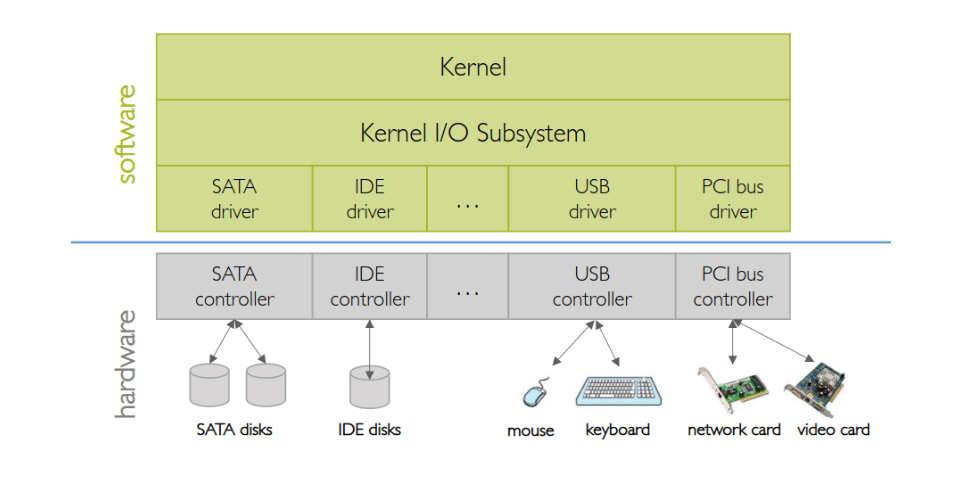
\includegraphics[width=0.6\textwidth,keepaspectratio]{{im/1_3}}
        \caption{Alcuni dei componenti di un semplice personal computer}    
    \end{center}
    \end{figure}

    \subsubsection{System Bus}
    Inizialmente veniva usato un unico bus per gestire tutto il traffico. Combina le funzioni di: 
    \begin{itemize}
        \item Data bus effettivo di informazioni
        \item Address bus per determiare dove tali informazioni devono essere inviate
        \item Control bus per indicare quali operazioni dovrebbero essere eseguite
    \end{itemize}
    Sono stati aggiunti più bus dedicati per gestire il traffico da CPU a memoria e I/O, PCI, SATA, USB, ecc.
    
    \subsubsection{Dispostivi di I/O}
    Ogni dispositivo I/O è composto da due parti fondamentali il dispositivo fisico stesso e il controller del dispositivo (chip o set di chip che controllano una famiglia di dispositivi fisici).\\
    Il sistema operativo comunica con un controller del dispositivo utilizzando un driver di dispositivo specifico.\\
    La communicazione con i "Dispositivi di Controllo" ciacun controller del dispositivo ha un numero di registri dedicati per comunicare con esso:
    \begin{itemize}
        \item \textbf{Registri di stato}: forniscono alla CPU informazioni sullo stato del dispositivo I/O (ad esempio, inattivo, pronto per l'input, occupato, errore, transazione completata)
        \item \textbf{ Registri di configurazione/controllo}: utilizzati dalla CPU per configurare e controllare il dispositivo
        \item \textbf{Registri dei dati}: utilizzati per leggere o inviare dati al dispositivo I/O
    \end{itemize}
    La CPU riesce ad indirizzare mettendo l'address di un byte di memoria nel address bus, specficando il segnale \texttt{READ} sul controllo del bus. Alla fine, la RAM risponderà con il contenuto della memoria sul Data bus.
    
    La CPU può comunicare con un controller del dispositivo in due modi:
    \begin{itemize}
        \item I/O mappati alle porte che fanno riferimento ai registri del controller utilizzando un I/O separato
        spazio degli indirizzi. \\Il registro di ciascun controller del dispositivo I/O è mappato su una porta specifica (indirizzo).\\
        Richiede classi speciali di istruzioni CPU (ad es. IN/OUT). L'istruzione \texttt{IN} legge da un dispositivo I/O, mentre \texttt{OUT} scrive. Quando si usano le istruzioni IN o OUT, l' \texttt{M/\#IO} non viene asserito, quindi la memoria non risponde e il chip I/O sì.
        \item I registri del controller del Memory-Mapped I/O utilizzano lo stesso spazio di indirizzamento utilizzato dalla memoria principale.\\Il Memory-mapped I/O "spreca" parte dello spazio degli indirizzi ma non necessita di istruzioni speciali. Per le porte del dispositivo I/O della CPU sono proprio come i normali indirizzi di memoria. La CPU utilizza istruzioni simili a \texttt{MOV} per accedere ai registri del dispositivo I/O. In questo modo viene asserito l' \texttt{M/\#IO} indicando l'indirizzo richiesto dalla CPU riferito alla memoria principale
    \end{itemize}
    Per eseguire le attività di I/O, vengono utilizzate due modalità di gestione:
    \begin{itemize}
        \item Polling
        \item La CPU periodicamente verifica lo stato dei task delle attività di I/O
        \item Interrupt-driven dove la CPU riceve un segnale di interrupt dal controller una volta che la task I/O viene completata
        \item La CPU riceve un interrupt dal controller (device o DMA \footnote{Direct Memory Access}) una volta finito il task dell'I/O (con successo o in modo anomalo)
        \item La CPU svolge il lavoro effettivo di spostamento dei dati
        \item La CPU delega il lavoro a un controller DMA dedicato
    \end{itemize}

\subsubsection{Processori}
La CPU preleva le istruzioni della memoria (esegue il \textbf{fetch}) e le esegue. La CPU si occupa poi di decodificarla per determinare il tipo e gli operandi , eseguirla e poi prelevare, decodificare ed eseguire le successive. Poichè accedere alla memoria richiede molte risorse tutte le CPU contengono all'interno dei \textbf{registri}  per memorizzare variabili importanti o risultati temporanei. Oltre ai registri i computer contengono il \textbf{program counter (PC)}, contente l'indirizzo di memoria in sui si trova la successiva istruzione da seguire, dopodichè viene il PC viene aggiornato per posizionarsi sulla successiva. \\
Un altro registro è lo \textbf{stack pointer} che punta alla cima dello stack attuale. Un altro registro è il \textbf{program status word (PSW)} che contiene i bit di condizione, impostati da istruzioni di confronto, la prorità della CPU, la modalità (kernel o utente) e altri bit di controllo. 
Nelle architetture più moderne, vengono implementati più livelli di protezione, detti \textbf{protection rings}. Ogni ring aggiunge restrizioni sulle istruzioni eseguibili dalla CPU.
\begin{figure}[hbt]
    \begin{center}
        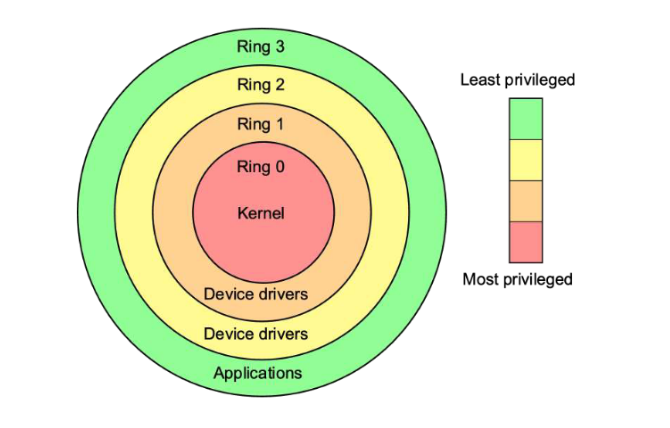
\includegraphics[width=0.5\textwidth,keepaspectratio]{{im/ring}}
        \caption{Protection Rings}    
    \end{center}
    \end{figure}

Un modo semplice per avere una protezione alla memoria è quello di avere due registri dedicati:
\begin{itemize}
    \item \textbf{Base} $\rightarrow$ contenente il primo address di partenza 
    \item \textbf{Limite} $\rightarrow$ contenente l'ultimo address valido 
\end{itemize}
Il sistema operativo carica i rigistri di base e limite all'avvio del programma mentre la CPU controlla che ogni indirizzo di memoria a cui fa riferimento il programma utente rientri tra i valori base e limite.


Per ottenere servizi dall'OS un programma utente deve fare una \textbf{system call (chiamata di sistema)} che entra nel kernel e richiama l'OS. Quando il lavoro è stato completato il controllo è restituito al programma utente.\\

L'istruzione \texttt{TRAP} cambia la modalità da utente a kernel e avvia l'OS. 
\begin{itemize}
    \item System call (software \texttt{TRAP}), ossia la richiesta di un servizio dell'OS, svolte in modo sincrono e innescate dai software
    \item Exception (fault), ossia la gestione di errori dovuti ad eventi inattesi, svolte in modo sincrono e innescate dai software
    \item Interrupt, ossia il completamento di una richiesta in attesa, svolte in modo asincrono e innescate dall'hardware
\end{itemize}

Esistono sei categorie importanti di System call:
\begin{itemize}
    \item \textbf{Gestione dei processi} include \texttt{end}, \texttt{abort}, \texttt{load}, \texttt{execute}, creazione e terminazione di processi, get/set attributi di processi, attesa, signal event, e allocazione di memoria libera. Quando un processo si interrompe o si interrompe, è necessario avviarne o riprenderne un altro. Quando i processi si arrestano in modo anomalo, potrebbe essere necessario fornire core dump e/o altri strumenti diagnostici o di ripristino
    \item \textbf{Gestione dei file} crea file, elimina file, apri, chiudi, leggi, scrivi, riposiziona, ottieni attributi di file e imposta attributi di file. Queste operazioni possono essere supportate anche per directory e file ordinari. L'effettiva struttura della directory può essere implementata utilizzando file ordinari sul file system o tramite altri mezzi (ne parleremo più avanti)
    \item \textbf{Gestione dei dispositivi} include dispositivi di richiesta, dispositivi di rilascio, lettura, scrittura, riposizionamento, recupero/impostazione degli attributi del dispositivo e collegamento o scollegamento logico dei dispositivi. I dispositivi possono essere fisici (ad es. unità disco) o virtuali/astratti (ad es. file, partizioni e dischi RAM). Alcuni sistemi rappresentano i dispositivi come file speciali nel file system, in modo che l'accesso al "file" richieda il driver di dispositivo del sistema operativo appropriato. E.g la directory \texttt{/dev} su qualsiasi sistema \texttt{UNIX}
    \item \textbf{Informazioni di sistema} include le chiamate per ottenere/impostare l'ora, la data, i dati di sistema e gli attributi di processo, file o dispositivo. I sistemi possono anche fornire la possibilità di eseguire il dump della memoria in qualsiasi momento. Programmi a passo singolo che interrompono l'esecuzione dopo ogni istruzione e tracciano
    il funzionamento dei programmi (debug). 
    \item \textbf{Communicazione} include creazione/eliminazione di connessioni di comunicazione, invio/ricezione di messaggi, trasferimento di informazioni sullo stato e collegamento/scollegamento di dispositivi remoti. Esisono due modelli di comunicazione: 
    \begin{itemize}
        \item \textbf{scambio di messaggi}\footnote{Nota: Più semplice e facile (in particolare per le comunicazioni tra computer) e generalmente appropriato per piccole quantità di dati\\}, il modello di trasmissione dei messaggi deve supportare le chiamate a:
        \begin{itemize}
            \item Identificare un processo remoto e/o un host con cui comunicare
            \item Stabilire una connessione tra i due processi
            \item Aprire e chiudere la connessione secondo necessità
            \item Trasmettere messaggi lungo la connessione
            \item Attendere i messaggi in arrivo, in stato di blocco o non blocco
            \item Eliminare la connessione quando non è più necessaria
        \end{itemize}
        \item \textbf{memoria condivisa}\footnote{Più veloce e generalmente l'approccio migliore in cui devono essere condivise grandi quantità di dati. Ideale quando la maggior parte dei processi deve leggere i dati anziché scriverli}, il modello di memoria condivisa deve supportare le chiamate a:
        \begin{itemize}
            \item  Creare e accedere alla memoria condivisa tra processi (e thread) 
            \item Fornire meccanismi di blocco che limitano l'accesso simultaneo
            \item Liberare memoria condivisa e/o allocarla dinamicamente secondo necessità
        \end{itemize}
    \end{itemize}
\end{itemize}

\subsubsection{Protezione delle system call}
Fornisce meccanismi per controllare quali utenti/processi hanno accesso a quali risorse di sistema. Le chiamate di sistema consentono di regolare i meccanismi di accesso secondo necessità. Agli utenti non privilegiati può essere concesso temporaneamente un accesso elevato autorizzazioni in circostanze specifiche. 
Quando un programma utente richiede l'esecuzione di una syscall tramite un'API fornita dal sistema operativo, tale richiesta viene prima convertita in linguaggio macchina, per poi venir gestita dal \textbf{System call Handler}, il quale si occuperà di salvare lo stato precedente dei registri, i quali verranno poi alterati durante l'esecuzione della syscall, per poi essere ripristinati. 

\subsubsection{Passaggio di parametri}
Esistono tre metodi usati per passare parametri :
\begin{itemize}
    \item Salvare i parametri in registri
    \item Salvare parametri in \texttt{block} o \texttt{table} di un'area di memoria dedicata
    \item Parametri inseriti nello stack dal programma e estratti dallo stack dal sistema operativo (più complessi a causa dei diversi spazi degli indirizzi)
\end{itemize}
I metodi block e stack non limitano il numero o la lunghezza dei parametri passati
\begin{figure}[hbt]
    \begin{center}
        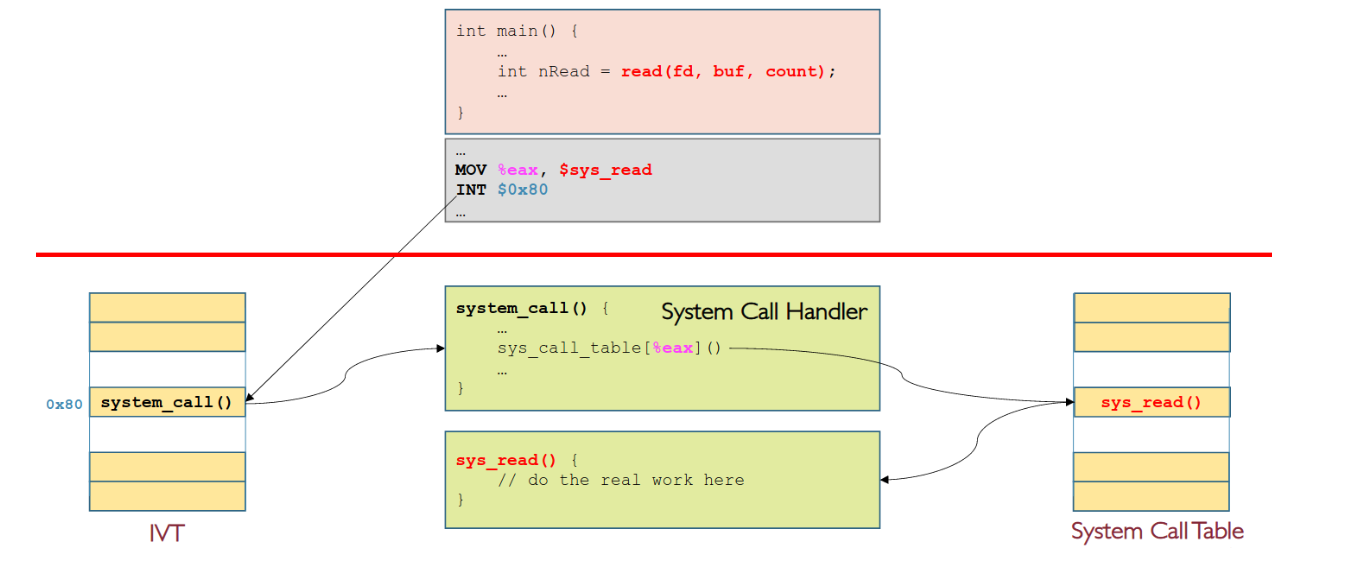
\includegraphics[width=0.9\textwidth,keepaspectratio]{{im/ivt}}
        \caption{System call Handler}    
    \end{center}
    \end{figure}
\subsubsection{Timer, Istruzioni atomiche, Virtual Memory}
Il timer è una funzionalità hardware per abilitare la scheduling della CPU. Nei sistemi multi-tasking, permette alla CPU di non essere monopolizzata da processi "egoistici". Il timer genera un interrupt e ad ogni sua interruzione, lo scheduler della CPU prende il sopravvento e decide quale processo da eseguire successivamente.\\
Gli interrupt possono verificarsi in qualsiasi momento e interferire con i processi in esecuzione e l'OS deve essere in grado di sincronizzare le attività di cooperazione, simultanee processi, garantire che brevi sequenze di istruzioni (ad es. lettura-modifica-scrittura) vengano eseguite atomicamente da disabilitare gli interrupt prima della sequenza e riabilitarli successivamente. \\
La virtualizzazionde della memoria è un'astrazione (dell'effettiva memoria principale fisica) e conferisce ad ogni processo l'illusione che la memoria fisica sia solo contigua spazio degli indirizzi (spazio degli indirizzi virtuali). Permette di eseguire programmi senza che vengano caricati interamente nella memoria principale. Può essere implementata sia in HW (\textbf{MMU}) che in SW (OS).
\begin{itemize}
    \item \textbf{MMU}, associa gli indirizzi virtuali a quelli fisici tramite una tabella delle pagine gestita dal sistema operativo. Utilizza una cache denominata Translation Look-aside Buffer (TLB) con "mappature recenti" per ricerche più rapide. Il sistema operativo deve sapere quali pagine sono caricate nella memoria principale e quali su disco
    \item Il sistema operativo è responsabile della gestione degli spazi di indirizzi virtuali
\end{itemize}


\begin{figure}[hbt]
    \begin{center}
        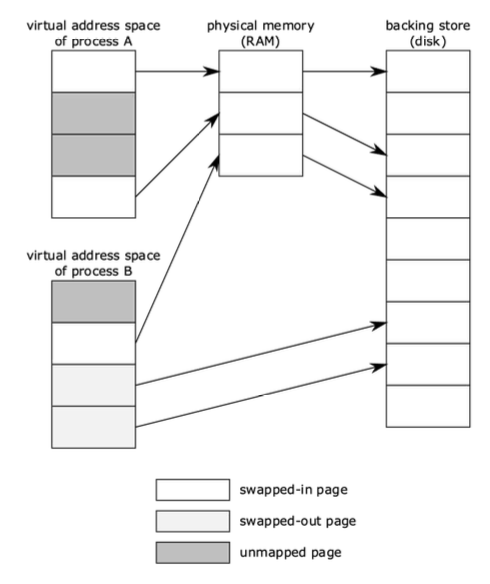
\includegraphics[width=0.3\textwidth,keepaspectratio]{{im/virtualm}}
        \caption{Virtual vs. Physical Address Space}    
    \end{center}
    \end{figure}

Lo spazio degli indirizzi virtuali è tipicamente suddiviso in blocchi contigui della stessa dimensione (ad esempio, 4 KiB), chiamati pagine (\textbf{pages}). Ciascuna pagina che non sono caricate nella memoria principale vengono memorizzate su disco.

\pagebreak

\subsection{Progettazione e implementazione del sistema operativo}
La struttura interna dei diversi sistemi operativi può variare notevolmente e gli obiettivi del sistema è facilare l'usabilità rispetto al progettare/implementare. È fondamentale separare le politiche dai meccanismi della policy ovvero \textbf{cosa} sarà fatto e il meccanismo che indica \textbf{come} farlo.
Il disaccoppiamento della logica della politica dal meccanismo sottostante è un principio di progettazione generale nell'informatica, in quanto migliora il sistema:
\begin{itemize}
    \item flessibilità: l'aggiunta e la modifica delle politiche possono essere facilmente supportate
    \item riusabilità: i meccanismi esistenti possono essere riutilizzati per implementare nuove politiche 
    \item stabilità: l'aggiunta di una nuova politica non destabilizza necessariamente il sistema    
\end{itemize}
Le modifiche ai criteri possono essere facilmente regolate senza riscrivere il codice.

I primi sistemi operativi sviluppati in linguaggio assembly, e uno dei vantaggi era il controllo diretto sull'HW (alta efficienza) mentre uno svantaggio può essere il legame con uno specifico HW (bassa portabilità). Oggi abbiamo un misto di linguaggi e ai livelli più bassi troveremo assembly il corpo principale in C e i programmi di sistema in C, C++, linguaggi di scripting come PERL, Python, ecc.\\
Il sistema operativo dovrebbe essere suddiviso in sottosistemi separati, ciascuno con compiti, input/output e caratteristiche prestazionali accuratamente definiti. Esistono vari modi di strutturare un sistema operativo: 

\begin{itemize}
    \item \textbf{Struttura semplice}, dove non vi è alcun sottosistema e non vi è separazione tra kernel e user mode (esempio: il sistema MS-DOS). Semplice da implementare ma estremamente insicuro e poco rigido.
    \item  \textbf{Struttura a Kernel Monolitico}, dove l'intero sistema operativo opera in kernel mode e solo i software utente lavorano in user mode (esempio: il sistema UNIX). Semplice da implementare ed efficiente, ma ancora poco sicuro e rigido
    \item \textbf{Struttura a livelli} (come MULTICS) dove l'OS è suddiviso in N livelli ed ogni livello L usa funzionalità implementate dal livello $L_{1}$ ed espone nuove funzionalità al livello L + 1. Per via della struttura a livelli, il sistema è molto modulare, portabile e semplice da debuggare, rendendo tuttavia più complessa per la comunicazione tra di essi.
    \item \textbf{Struttura a Microkernel}, dove il kernel contiene solo le funzionalità di base, mentre tutte le altre funzionalità dell'OS e i programmi utente vengono eseguiti in user mode. Tale struttura porta ad una maggiore sicurezza, affidabilità ed estensibilità, ma anche ad un'efficienza ridotta.
    \item \textbf{Struttura a Moduli del Kernel caricabili (LKM)}, dove l'OS utilizza dei moduli tramite cui accedere alle funzionalità del kernel
    \item \textbf{Sistema a Kernel Ibrido}, dove viene utilizzato un approccio intermedio al kernel monolitico e al microkernel, ottenendo i vantaggi di entrambi gli approcci
\end{itemize}
\pagebreak
%-------------------------------------------------------%
\section{Gestione dei Processi e thread}

Un programma è un file eseguibile che risiede nella memoria persistente (ad es. disco) e contiene solo l'insieme di istruzioni necessarie per eseguire un lavoro specifico. Un processo è l'astrazione del sistema operativo di un programma in esecuzione (unità di esecuzione). Il processo è dinamico, mentre un programma è statico (solo codice e dati). Diversi processi possono eseguire lo stesso programma (ad esempio, multiple istanze di Google Chrome) ma ognuna ha il proprio stato. Un processo esegue un'istruzione alla volta, in sequenza. \\

Il sistema operativo fornisce la stessa quantità di spazio di indirizzi virtuali a ciascun processo. Lo spazio degli indirizzi virtuali è un'astrazione dello spazio degli indirizzi della memoria fisica. L'intervallo di indirizzi virtuali validi che un processo può generare dipende dalla macchina. Avremo perciò:
\begin{itemize}
    \item \textbf{Text} contenente le istruzioni dell'eseguibile
    \item \textbf{Data} Variabili globali e statiche inizializzate
    \item \textbf{BSS} variabile globale e statica (non inizializzata o inizializzata a 0)
    \item \textbf{Stack} Struttura LIFO utilizzata per memorizzare tutti i dati necessari a una chiamata di funzione (stack frame)
    \item \textbf{Heap} usata per l'allocazione dinamica
\end{itemize}

\begin{figure}[hbt]
    \begin{center}
        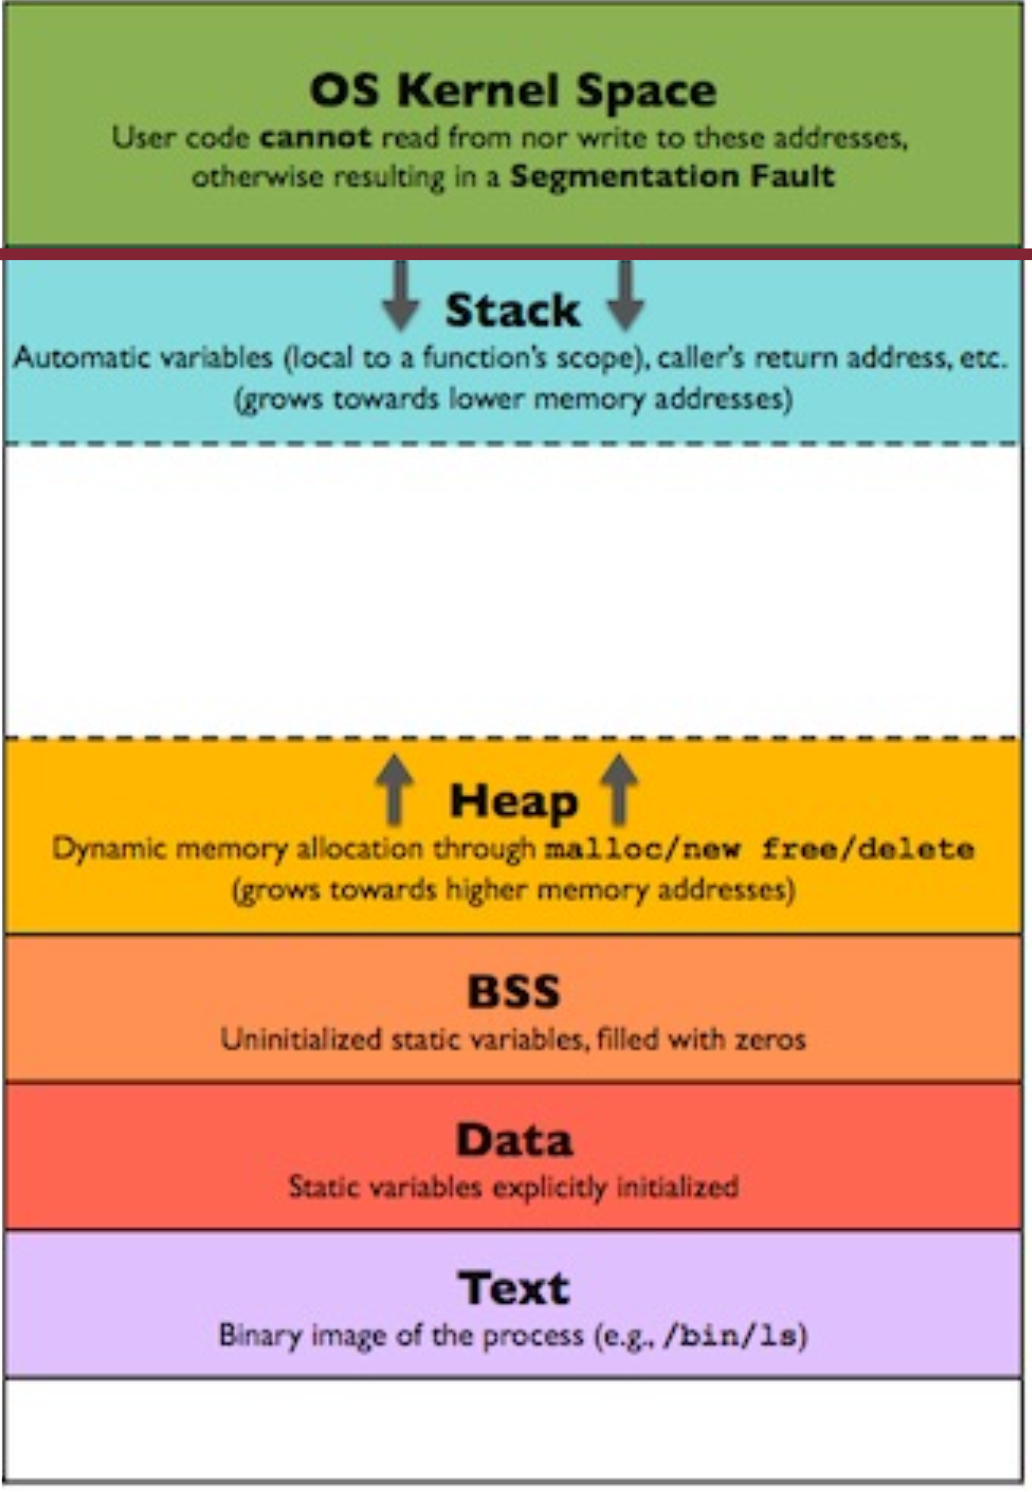
\includegraphics[width=0.3\textwidth,keepaspectratio]{{im/virtualaddress}}
        \caption{Virtual Address Space Layout}    
    \end{center}
    \end{figure}

Sullo stack sono definite due operazioni: \textbf{push} e \textbf{pop}. Il push viene usato per inserire degli elementi, mentre pop per rimuoverli. Usa un registro dedicato (e.g \texttt{esp}) il cui contenuto è l'indirizzo nella memoria principale della parte superiore dello stack. La memoria dello stack cresce convenzionalmente dall'alto verso il basso, cioè dagli indirizzi di memoria più alti a quelli più bassi. Ogni funzione utilizza una porzione dello stack, chiamata \textbf{stack frame} e in ogni momento possono esistere contemporaneamente più stack frame, a causa di diverse chiamate di funzioni nidificate, ma solo una è attiva.
Lo stack frame per ogni funzione è diviso in tre parti:
\begin{itemize}
    \item parametri della funzione + indirizzo di ritorno
    \item back-pointer allo stack frame precedente
    \item variabili locali
\end{itemize}
Il primo è impostato dal chiamante, il secondo e il terzo vengono impostati dal chiamato. Il puntatore \texttt{esp} viene sempre aggiornato man mano che lo stack cresce ed è difficile per il chiamato accedere ai parametri effettivi senza un riferimento fisso nello stack. Per risolvere questo problema invece di utilizzare un singolo puntatore in cima allo stack usa un puntatore aggiuntivo alla parte inferiore (base) dello stack (\texttt{\%ebp}) lascia che \texttt{esp} sia libero di cambiare tra diverse chiamate di funzione, mentre tiene \texttt{\%ebp} fissato all'interno di ogni stack frame. \\

\begin{figure}[hbt]
    \begin{center}
        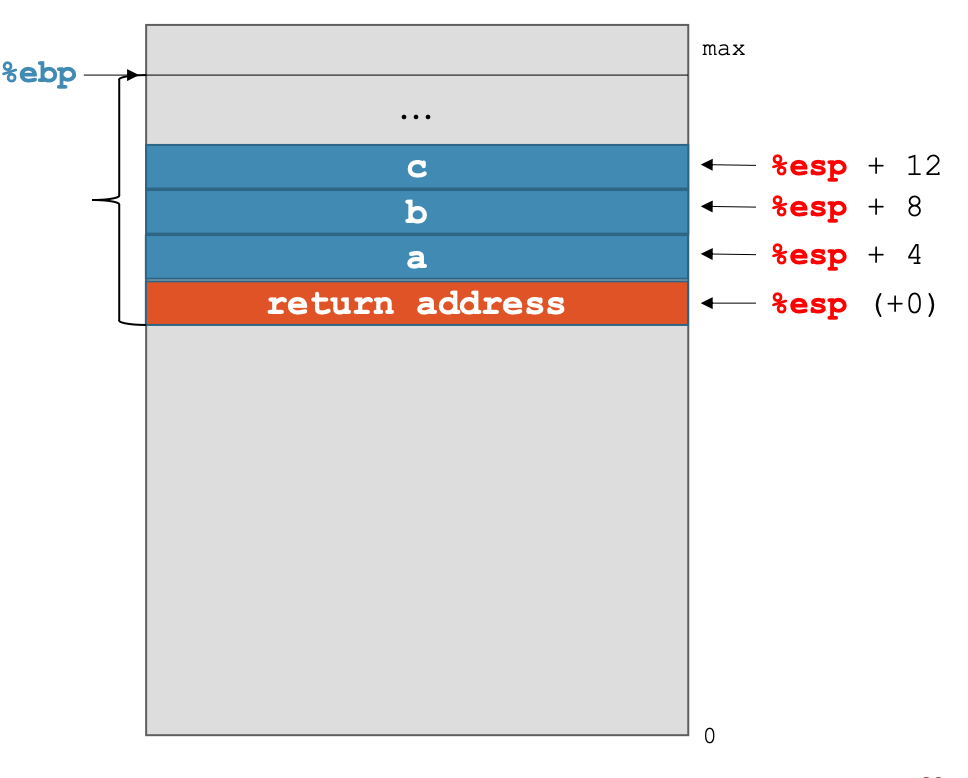
\includegraphics[width=0.5\textwidth,keepaspectratio]{{im/ebp}}
        \caption{Function Parameters + Return}    
    \end{center}
    \end{figure}
\subsection{Stato di esecuzione del processo}
In ogni momento un processo può trovarsi in uno dei seguenti cinque stati:
\begin{itemize}
    \item \textbf{New}, il processo appena avviato
    \item \textbf{Ready}, il processo è pronto per essere eseguito ma attende di essere programmato sulla CPU
    \item \textbf{Running}, il processo sta effettivamente eseguendo istruzioni sulla CPU 
    \item \textbf{Waiting}, il processo è sospeso in attesa che una risorsa sia disponibile o un
    evento da completare/verificare (ad es. input da tastiera, accesso al disco, timer, ecc.)
    \item \textbf{Terminated}, il processo è terminato e il sistema operativo può distruggerlo
\end{itemize}

\begin{figure}[hbt]
    \begin{center}
        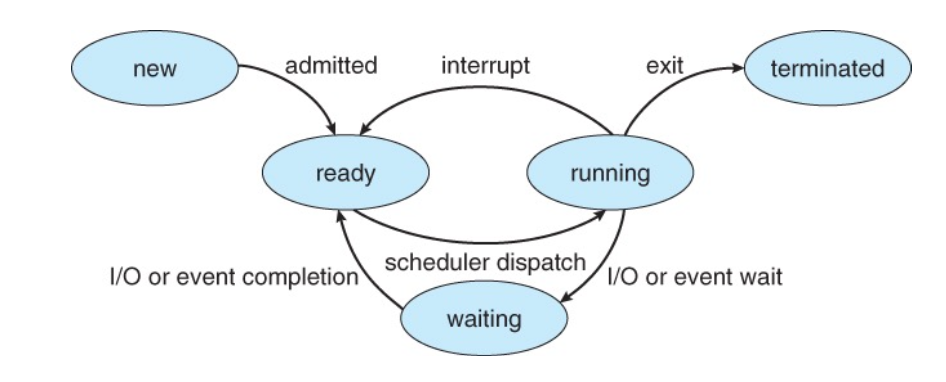
\includegraphics[width=0.7\textwidth,keepaspectratio]{{im/diagramma}}
        \caption{Process Execution State Diagram}    
    \end{center}
    \end{figure}

Durante l'esecuzione, il processo passa da uno stato all'altro in base alle azioni del programma (ad esempio, chiamate di sistema) come azioni del sistema operativo (ad es. scheduling) o azioni esterne (ad es. interruzioni).\\ 

La maggior parte delle chiamate di sistema (ad esempio quelle di I/O) sono bloccanti. Il processo chiamante (spazio utente) non può fare nulla fino al ritorno della chiamata di sistema.\\
 Il sistema operativo (spazio del kernel) si occupa di:
\begin{itemize}
    \item impostare il processo corrente in uno stato di attesa (ovvero, in attesa del ritorno della chiamata di sistema)
    \item  pianifica un diverso processo pronto per evitare che la CPU sia inattiva
\end{itemize} 
Una volta che la chiamata di sistema ritorna, il processo precedentemente bloccato è pronto per essere schedulato nuovamente per l'esecuzione.\footnote{NOTA: l'intero sistema non è bloccato, solo il processo che ha richiesto la chiamata bloccata è!\\}\\
Lo stato del processo è costituito da: 
\begin{itemize}
    \item il codice del programma in esecuzione
    \item i dati statici del programma in esecuzione
    \item il program counter (PC) che indica la prossima istruzione da eseguire
    \item Registri CPU
    \item la catena di chiamate del programma (stack) insieme ai puntatori di frame e stack
    \item lo spazio per l'allocazione dinamica della memoria (heap) e al suo puntatore, le risorse in uso (ad es. file aperti)
    \item lo stato di esecuzione del processo (pronto, in esecuzione, ecc.)
\end{itemize}

\subsection{Process Control Block (PCB)}
Il \textbf{PCB} (o detto anche Tabella dei Processi), è la struttura dati principale utilizzata dal sistema operativo per tenere traccia di qualsiasi processo. Il PCB tiene traccia dello stato di esecuzione e della posizione di un processo. Il sistema operativo assegna un nuovo PCB alla creazione di un processo e lo inserisce in una coda di stato e viene deallocato non appena termina il processo associato. \\Associata a ogni classe di I/O c'è una posizione (solitamente in una collocazione fissa vicino alla base della memoria) chiamata \textbf{vettore di interrupt}\footnote{In informatica, un interrupt vector (vettore delle interruzioni) è un indirizzo di memoria del gestore di interrupt, oppure un indice ad un array, chiamato interrupt vector table, il quale può essere implementato tramite una dispatch table. La tabella degli interrupt vector contiene gli indirizzi di memoria dei gestori di interrupt. Quando si genera una interruzione, il processore salva il suo stato di esecuzione con il context switch, ed inizia l'esecuzione del gestore di interruzione all'interrupt vector (questo procedimento avviene quando l'interruzione ha carattere sincrono). Infatti vi è una wait instruction (istruzione d'attesa) che obbliga la CPU ad effettuare cicli vuoti fino a che non arriva il prossimo interrupt. Nel caso in cui si dovesse verificare una interruzione asincrona il programma provvede a lanciare un interrupt con la richiesta di I/O e nell'attesa del dato continua ad effettuare operazioni logico-aritmetiche. Quando arriverà nel momento in cui gli servirà il risultato si fermerà e inizierà ad aspettare. L'I/O asincrono serve a far sì che alcuni programmi possano anticipare la richiesta di un dato così nel caso in cui esso dovesse servire lo possono già utilizzare. Fonte: Wikipedia}. Contiene l'indirizzo della procedura di servizio dell'interrupt. Ad ogni interrupt il computer salta all'indirizzo specificato nel vettore dell'interrupt. 
Il PCB contiene:
\begin{itemize}
    \item Stato del processo pronto, in attesa, in esecuzione, ecc.
    \item Numero di processo (ovvero identificatore univoco)
    \item Program Counter (PC) + Stack Pointer (SP) + registri di uso generale 
    \item Informazioni sullo scheduling della CPU priorità e puntatori alle code di stato 
    \item Informazioni sulla gestione della memoria tabelle delle pagine
    \item Informazioni sull'account, ossia il  tempo utilizzato dalla CPU del kernel e dell'utente, stato I/O del proprietario 
    \item Elenco dei file aperti
\end{itemize}
\begin{figure}[hbt]
    \begin{center}
        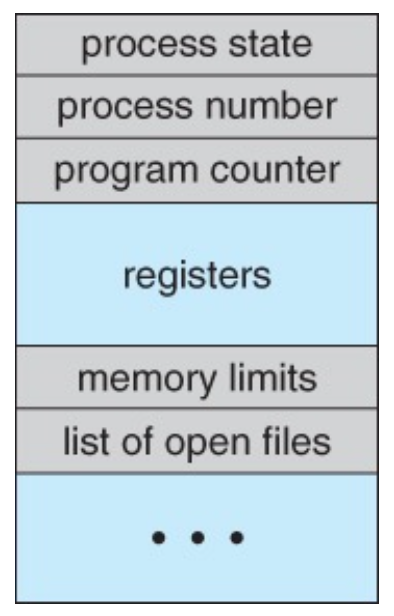
\includegraphics[width=0.2\textwidth,keepaspectratio]{{im/PCB}}
        \caption{Process Execution State Diagram}    
    \end{center}
    \end{figure}
\pagebreak
\subsection{Creazione di processi}
I processi possono creare altri processi tramite specifiche chiamate di sistema. Il processo creatore è chiamato genitore del nuovo processo, chiamato figlio. Il genitore condivide risorse e privilegi con i suoi figli. Un genitore può aspettare che un figlio finisca o continuare in parallelo.\\
A ogni processo viene assegnato un identificatore intero (noto anche come identificatore di processo o PID) e per ogni processo viene memorizzato anche il PID genitore (PPID).\\
Sui tipici sistemi UNIX lo scheduler del processo è denominato \texttt{sched} e riceve il PID 0. La prima cosa che fa all'avvio del sistema è lanciare \texttt{init}, che dà a quel processo il PID 1. Successivamente \texttt{init} avvia tutti i daemons di sistema e i login degli utenti e diventa il genitore ultimo di tutti gli altri processi. I processi vengono creati attraverso la chiamata di sistema \texttt{\texttt{fork()}}.\\

Tutti i processi sono uguali. L'unico indizio di gerarchia dei processi è che quando viene creato un processo, al genitore viene dato uno speciale gettone o token (detto \textbf{handle}) che può controllare il figlio invalidando la gerarchia.\\
\begin{figure}[hbt]
    \begin{center}
        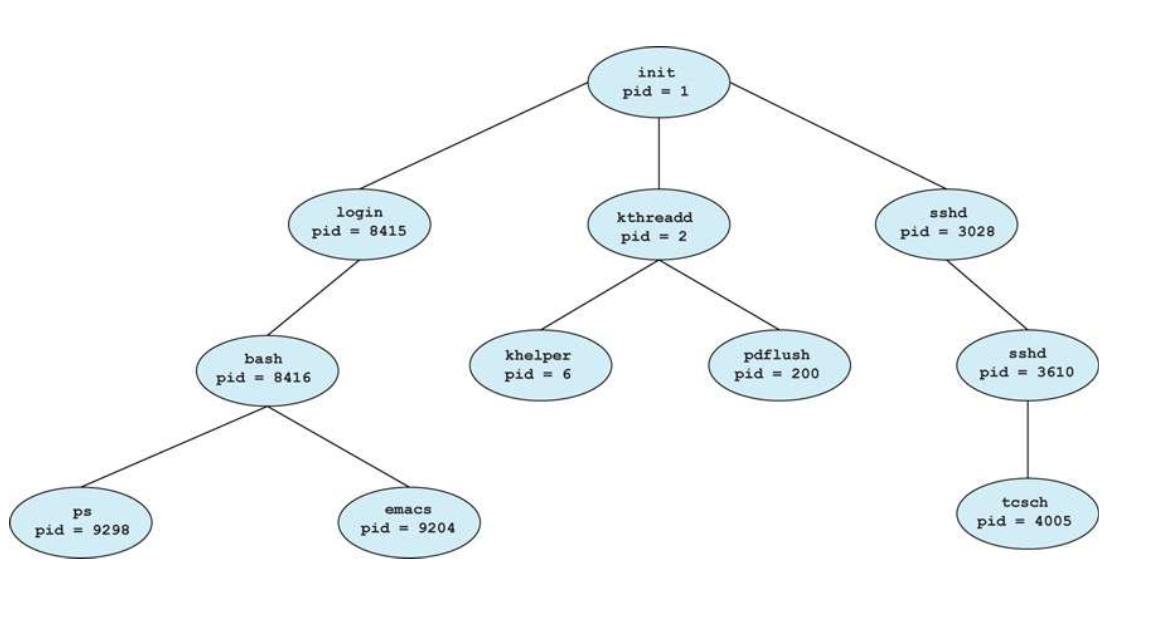
\includegraphics[width=0.7\textwidth,keepaspectratio]{{im/creazioneProcessi}}
        \caption{Process Creation: UNIX/Linux}    
    \end{center}
    \end{figure}
\pagebreak
\subsubsection{Risorse del padre vs figlio}
Abbiamo due possibilità per lo spazio degli indirizzi del figlio rispetto al genitore:
\begin{itemize}
    \item Il bambino può essere un duplicato esatto del genitore, condividendo lo stesso programma e gli stessi segmenti di dati in memoria
    \item Ciascuno avrà il proprio PCB, inclusi program counter, registri e PID 
    \item Questo è il comportamento della chiamata di sistema \texttt{fork()} in UNIX
    \item Il processo figlio può avere un nuovo programma caricato nel suo spazio degli indirizzi, con tutti i nuovi segmenti di codice e dati
    \item In Windows le chiamate di sistema saranno create con il comando \texttt{spawn()} 
    \item I sistemi UNIX implementano ciò come secondo passaggio, utilizzando la chiamata di sistema \texttt{exec}.
\end{itemize}
\subsubsection{Esecuzione del padre vs figlio}
Abbiamo due opzioni per il processo genitore dopo aver creato il figlio:
\begin{itemize} 
    \item Attendere che il processo figlio termini prima di procedere emettendo un \texttt{wait} chiamata di sistema, per un figlio specifico o per qualsiasi figlio
    \item Oppure eseguire contemporaneamente al figlio, continuando l'elaborazione senza essere bloccato (quando una shell UNIX esegue un processo come attività in background utilizzando "\&")
\end{itemize}

Consideriamo ora questo esempio:
\begin{lstlisting}
    #include <sys/types.h>
    #include <stdio.h>
    #include <unistd.h>
    int main(){
        pid_t pid;
        /* fork a child process */
        pid = \texttt{fork()};
        if (pid < 0) { 
            /* if the returned PID is < 0, an error occurred */
            fprintf(stderr, "Fork Failed");
            exit(-1); 
        }
        else if (pid == 0) {
        /* execute child process code */
            execlp("/bin/ls", "ls", NULL);
        }
        else {
        /* execute parent process code */
            ...
            /* wait for child to terminate */
            wait(NULL)
            printf("Child terminated");
            exit(0); 
    }
}
\end{lstlisting}

\begin{figure}[hbt]
    \begin{center}
        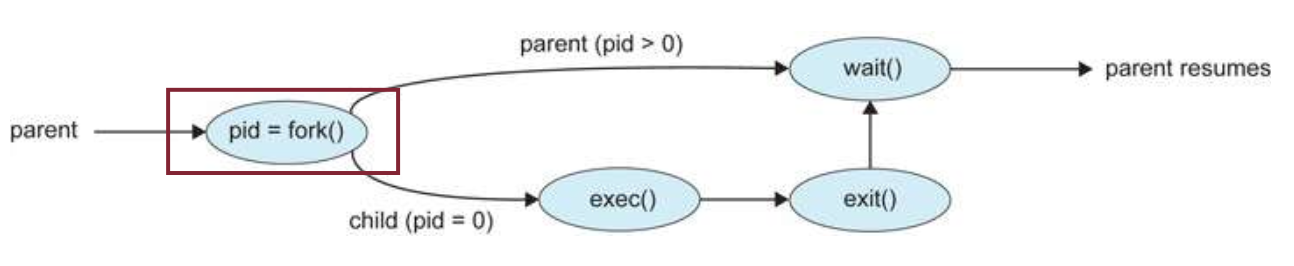
\includegraphics[width=0.7\textwidth,keepaspectratio]{{im/p1}}
        \caption{Albero decisionale del primo esempio}    
    \end{center}
    \end{figure}
\pagebreak
Consideriamo ora quest'altro esempio:
\begin{lstlisting}
    int pid = \texttt{fork()};
    if(pid == 0) {      // A's child (B)
        pid = \texttt{fork()};
        
    if(pid == 0) {      // B's child (C)
        ...
        execlp(...);
    }
    else { // B 
        ...
    } 
}
else { // A 
    ...
}
\end{lstlisting}
\begin{figure}[hbt]
    \begin{center}
        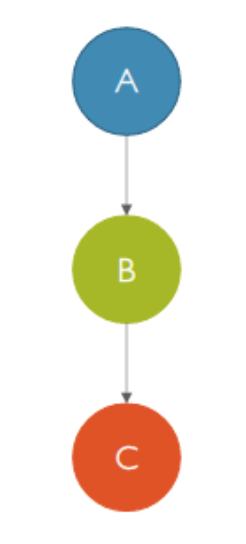
\includegraphics[width=0.15\textwidth,keepaspectratio]{{im/p2}}
        \caption{Albero decisionale del secondo esempio}    
    \end{center}
\end{figure}

\pagebreak

Consideriamo ora questo esempio:
\begin{lstlisting}
    int pid = \texttt{fork()};
    if(pid == 0) {          // A's child (B)
        ...
        execlp(...);
    }
    else { // A
        pid = \texttt{fork()};
        if(pid == 0) {      // A's child (C)
            ...
            execlp(...);
        }
    }
\end{lstlisting}
\begin{figure}[hbt]
    \begin{center}
        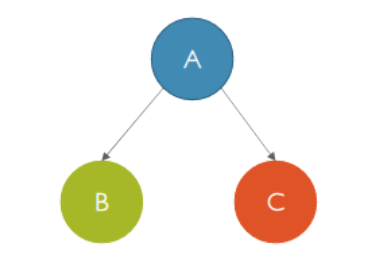
\includegraphics[width=0.25\textwidth,keepaspectratio]{{im/p3}}
        \caption{Albero decisionale del secondo esempio}    
    \end{center}
\end{figure}

Consideriamo ora quest'altro esempio:
\begin{lstlisting}
    for(int i=0;i<n;i++) {
        if(\texttt{fork()} == 0) { // A0's child
            ...
            execlp(...);
        }
  }
  // back in the parent A0
  // wait for all children to terminate

  for(int i=0;i<n;i++) {
      wait(NULL);
  }
\end{lstlisting}
\begin{figure}[hbt]
    \begin{center}
        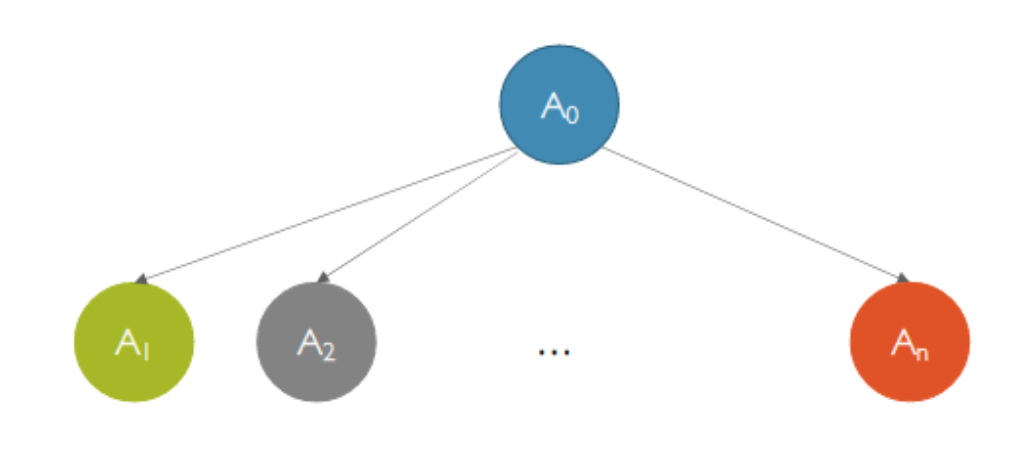
\includegraphics[width=0.2\textwidth,keepaspectratio]{{im/p4}}
        \caption{Albero decisionale del secondo esempio}    
    \end{center}
\end{figure}
Riepilogo delle chiamate di sistema viste:
\begin{itemize}
    \item \texttt{fork()} genera un nuovo processo figlio come copia esatta del genitore 
    \item \texttt{execlp} sostituisce il programma del processo corrente con il
    inserire il programma denominato
    \item \texttt{sleep} sospende l'esecuzione per un certo numero di secondi
    \item \texttt{wait}/\texttt{waitpid}  attende che uno o più processi specifici terminino l'esecuzione
\end{itemize}


\pagebreak

\subsection{Terminazione di processi}
I processi possono richiedere la propria terminazione effettuando la chiamata di sistema \texttt{exit}, tipicamente restituendo un \textit{int}. Questo \textit{int} viene passato al genitore se sta eseguendo un'attesa. Solitamente è 0 in caso di completamento con successo e un diverso da zero in caso di problemi.\\
I processi possono anche essere terminati dal sistema per una serie di motivi: 
\begin{itemize} 
    \item L'incapacità del sistema di fornire le risorse di sistema necessarie
    \item In risposta a un comando \texttt{kill} o ad un altro interrupt di processo non gestito
    \item Uscita normale (condizione volontaria)
    \item Uscita su errore (condizione volontaria)
    \item Terminato da un altro processo (condizione involontaria)
\end{itemize}
Un genitore può uccidere i suoi figli se il compito loro assegnato non è più necessario, il sistema però può consentire (o meno) al figlio di continuare senza un genitore. Sui sistemi UNIX, i processi orfani sono generalmente ereditati da \texttt{init}, che poi li uccide.\\

Quando un processo termina, tutte le sue risorse di sistema vengono liberate, i file aperti svuotati e chiusi, ecc. Lo stato di terminazione del processo dei tempi di esecuzione vengono restituiti al genitore se è in attesa che il figlio termini o \texttt{init} se il processo diventa orfano. \\

I processi sono detti \textbf{zombie} se stanno tentando di terminare ma non possono perché il loro genitore non li sta aspettando oppure ereditati da \texttt{init} come orfani e uccisi.

\subsection{Scheduling dei processi}

Gli obiettivi principali del sistema di schedulazione dei processi:
\begin{itemize} 
    \item mantenere la CPU sempre occupata
    \item fornire tempi di risposta "accettabili" per tutti i programmi, in particolare per quelli interattivi
\end{itemize}
Lo scheduler del processo deve soddisfare questi obiettivi implementando politiche adeguate per lo scambio dei processi dentro e fuori la CPU. Questi obiettivi però possono essere contrastanti, e ogni volta che il sistema operativo interviene per scambiare i processi, impiega tempo sulla CPU per farlo, che viene quindi "perso" dal fare qualsiasi lavoro produttivo utile.\\

Il sistema operativo mantiene i PCB di tutti i processi nelle code di stato. C'è una coda per ciascuno dei cinque stati in cui può trovarsi un processo e una per ogni dispositivo I/O (dove i processi attendono che un dispositivo diventi disponibile o consegni i dati). Quando il sistema operativo cambia lo stato di un processo, il PCB viene scollegato dalla coda corrente e spostato in quella nuova. Il sistema operativo può utilizzare criteri diversi per gestire ciascuna coda di stato. \\

La coda di esecuzione è vincolata dal numero di core disponibili sul sistema. Ogni volta, è possibile eseguire un solo processo su una CPU. Non esiste un limite teorico al numero di processi negli stati \texttt{new/ready/waiting/terminated}.\\

Esisono diversi scheduler (che in un sistema efficiente utilizza un mix tra questi):
\begin{itemize}
    \item Uno \textbf{scheduler a lungo termine} viene eseguito raramente ed è tipico di un sistema batch o di un sistema molto carico
    \item Uno \textbf{scheduler a breve termine} viene eseguito molto frequentemente (circa ogni 100 millisecondi) e deve sostituire molto rapidamente un processo dalla CPU e inserirne un altro
    \item Alcuni sistemi utilizzano anche uno \textbf{scheduler a medio termine}: quando i carichi del sistema diventano elevati, questo scheduler consente ai lavori più piccoli e più veloci di terminare rapidamente e liberare il sistema
\end{itemize}

\subsubsection{Il Context Switch}
Il \textbf{Context Switch} procedura utilizzata dalla CPU per sospendere il processo attualmente in esecuzione al fine di eseguirne uno pronto. È un'operazione molto costosa in quanto l'arresto del processo in corso implica il salvataggio di tutto il suo stato interno (PC, SP, altri registri, ecc.) al suo PCB e l'avvio di un processo pronto consiste nel caricare tutto il suo stato interno (PC, SP, altri registri, ecc.) dal suo PCB. \\
Il Context Switch si usa quando ci sono delle chiamate \texttt{TRAP}\footnote{richiesta di un servizio dell'OS, svolte in modo sincrono e innescate dai software\\} come system call, eccezioni, o interruzioni hardware. Ogni volta che arriva una \texttt{TRAP} la CPU ha il compito di creare uno stato di salvataggio dello stato corrente dei processi attivi. Passare alla modalità kernel per gestire l'interrupt ed eseguire un ripristino dello stato del processo interrotto. \\
Per evitare che i processi legati alla CPU monopolizzino la CPU, anche il Context Switch viene attivato tramite interrupt del timer hardware (\textbf{slice}).
Lo \textbf{slice} ha quantità massima di tempo tra due cambi di contesto per garantire che si verifichi almeno un cambio di contesto. Può accadere più frequentemente di così (ad esempio, a causa di richieste di I/O). Lo slice è facilmente implementabile in hardware tramite interrupt timer. E' un meccanismo utilizzato dai moderni sistemi operativi multitasking time-sharing per aumentare la reattività del sistema (pseudo-parallelismo). \footnote{Diverso invece quando si parla di \textbf{multiprocessore} che hanno due o più CPU che condividono la stessa memoria fisica, vero parallelismo hardware\\} \\
\subsubsection*{Il tempo nel Context Switch}
Il tempo impiegato per completare un cambio di contesto è solo tempo di CPU sprecato. Un intervallo di tempo inferiore comporta cambi di contesto più frequenti. Un intervallo di tempo maggiore comporta cambi di contesto meno frequenti. Ha anche il compito di minimizzare lo spreco di tempo della CPU, massimizzando quindi l'utilizzo e la reattività della CPU. 
\subsection{Communicazione dei processi}

I processi possono essere \textbf{indipendenti} o \textbf{cooperanti}:
\begin{itemize}
    \item Processi \textbf{indipendenti} operano contemporaneamente su un sistema e possono né influenzare né essere influenzati da altri processi
    \item I processi \textbf{cooperanti} possono influenzare o essere influenzati da altri processi al fine di raggiungere un compito comune
\end{itemize}

Possono esserci diversi processi che richiedono l'accesso allo stesso file (ad es pipeline). Abbiamo bisogno di questa cooperazione tra processi e ci sono diverse caratteristiche importanti. Abbiamo la \textbf{velocità} di calcolo è un problema che può essere risolta più velocemente se può essere suddiviso in sotto-attività da risolvere simultaneamente. La \textbf{modularità} definisce l'architettura più efficiente può essere quella di scomporre un sistema in moduli cooperanti. Infine abbiamo la \textbf{convenienza} infatti anche un singolo utente può essere multi-tasking, come modificare, compilare, stampare ed eseguire lo stesso codice in finestre diverse.
Ci sono due modi possibili per comunicare tra processi cooperanti:
\begin{itemize}
    \item \textbf{Memoria condivisa}\footnote{Per far sì che un processo possa richiedere un'area di memoria da condividere con altri processi c'è, ovviamente, necessità di effettuare una chiamata di sistema (a livello utente, non sarebbe possibile completare quest'operazione). Tuttavia, una volta "pagato questo prezzo iniziale", le interazioni successive tra processi che condividono un'area di memoria può avvenire senza ulteriori chiamate di sistema. \textbf{Fonte: il Prof}}
    \begin{itemize}
        \item Più complicato da configurare e non funziona altrettanto bene su più computer
        \item Più veloce una volta configurato, poiché non sono necessarie chiamate di sistema
        \item Preferibile quando (una grande quantità) di informazioni deve essere condivisa sullo stesso computer
    \end{itemize}
    \item \textbf{Scambio di messaggi} 
    \begin{itemize}
        \item Più semplice da configurare e funziona bene su più computer
        \item Più lento in quanto richiede chiamate di sistema (syscall) per ogni trasferimento di messaggi
        \item Preferibile quando la quantità e/o la frequenza dei trasferimenti di dati è piccola o quando sono multipli i computer sono coinvolti
    \end{itemize}
\end{itemize}

La memoria da condividere è inizialmente all'interno dello spazio degli indirizzi di un particolare processo e bisogna effettuare chiamate di sistema per rendere quella memoria pubblicamente disponibile ad altri processi.\\ Altri processi devono effettuare le proprie chiamate di sistema per collegare la memoria condivisa al proprio spazio degli indirizzi. \\
Il \textbf{Message Passing Systems} deve supportare almeno chiamate di sistema per l'invio e la ricezione di messaggi e stabilire un collegamento di comunicazione tra i cooperanti processi prima che i messaggi possano essere inviati.\\
\linebreak

Esistono però tre problemi da risolvere nello scambio di messaggi:\\

\begin{itemize}
    \item Comunicazione diretta o indiretta (es. naming) 
    \begin{itemize}
        \item Nella \textbf{Comunicazione diretta} il mittente deve conoscere il nome del destinatario a cui desidera inviare un messaggio. Deve conoscere anche il collegamento uno a uno tra ogni coppia mittente-destinatario per la comunicazione simmetrica e il destinatario deve conoscere anche il nome del mittente.
        \item La \textbf{Comunicazione indiretta} utilizza mailbox o porte condivise dove più processi possono condividere la stessa mailbox o porta. Solo un processo può leggere un determinato messaggio in una mailbox. Il sistema operativo deve fornire chiamate di sistema per creare ed eliminare mailbox e per inviare e ricevere messaggi da/per mailbox. 
    \end{itemize}
    \item Comunicazione sincrona o asincrona 
    \item Buffering automatico o esplicito
\end{itemize}
Scegliere se utilizzare o meno una queue per i messaggi:

\begin{itemize}
    \item \textbf{Zero capacity}, dove i messaggi non possono essere salvati in una queue, dunque il mittente rimane bloccato finché il destinatario non riceve il messaggio.
    \item \textbf{Bounded capacity}, dove vi è una queue di capienza predefinita, permettendo ai mittenti di non bloccarsi a meno che la queue non sia piena.
    \item \textbf{Unbounded capacity}, dove la queue ha teoricamente capienza infinita, implicando che i mittenti non debbano mai bloccarsi.
\end{itemize}


\subsection{Scheduling dei processi}
Definiamo come CPU burst lo stato in cui un processo è eseguito dalla CPU, mentre definiamo come I/O burst lo stato in cui un processo è in attesa che i dati vengano trasferiti dentro o fuori dal sistema.
In generale, ogni processo alterna costantemente tra CPU burst e I/O burst.\\
Lo scheduling dei processi è una \textbf{politica} che stabilisce quali processi devono essere eseguiti dalla CPU. Lo scheduler della CPU è un processo che, a seconda di una policy di scheduling stabilita, si occupa di selezionare un processo dalla ready queue da eseguire in ogni momento in cui la CPU è inattiva.
La struttura dati utilizzata per la ready queue e l'algoritmo usato per selezionare il processo successivo è basato su una queue FIFO (First In, First Out).

\begin{itemize}
    \item Concetti di base dello scheduling. Quasi tutti i programmi hanno alcuni cicli alternati di calcoli della CPU e attesa di I/O. Anche un semplice recupero dalla memoria principale richiede molto tempo rispetto alla velocità della CPU. (Consideriamo per ora la multiprogrammazione sui sistemi con un unico processore)
    \item Algoritmi di scheduling
    \item Concetti avanzati di scheduling.
\end{itemize} 

Ogni volta che la CPU diventa inattiva lo \textbf{scheduler} della CPU seleziona un altro processo dalla coda pronta per l'esecuzione successiva. La struttura dei dati per la coda pronta e l'algoritmo utilizzato per selezionare il processo successivo non sono però necessariamente basati su una coda FIFO. Le \textbf{decisioni di scheduling} della CPU avvengono in una delle quattro condizioni:
\begin{enumerate}
    \item Quando un processo passa dallo stato in \textbf{esecuzione} allo stato di \textbf{attesa}
    \item Quando un processo passa dallo stato in \textbf{esecuzione} allo stato \textbf{pronto}
    \item Quando un processo passa dallo stato di \textbf{attesa} allo stato \textbf{pronto}
    \item Quando un processo viene \textbf{creato} o \textbf{terminato}
\end{enumerate}

Nel 1° e il 4° caso è necessario selezionare un nuovo processo, mentre nel 2° e 3° caso si continua con il processo corrente o bisogna selezionarne uno nuovo. 
\subsection{Scheduling Preemptive e Non-Preemptive}
Un algoritmo di scheduling \textbf{non-preemptive} assegna la CPU a un processo e non lo interrompe finché non termina o finché non rilascia volontariamente la CPU. Ciò significa che un processo che richiede una quantità considerevole di tempo della CPU può bloccare altri processi che sono in attesa di esecuzione.\\ 

Un algoritmo di scheduling \textbf{preemptive}\footnote{Nota: uno scheduler preemptive viene comunque attivato dalle condizioni 1 e 4, poiché in tali casi deve comunque essere selezionato un processo.}, al contrario, consente al sistema operativo di interrompere l'esecuzione di un processo in qualsiasi momento per consentire l'esecuzione di un altro processo in coda. Questo significa che i processi con un tempo di esecuzione più breve possono essere eseguiti più rapidamente, anche se ci sono altri processi in attesa di esecuzione. 
\subsubsection{Problemi}
Preemption potrebbe causare problemi se si verifica mentre il kernel è impegnato nell'implementazione di una system call (ad esempio, l'aggiornamento dei dati critici del kernel strutture) oppure due processi condividono dati, uno può essere interrotto durante l'aggiornamento di strutture dati condivise. Ci sono però possibili \textbf{soluzioni}, si può fare in modo che il processo attenda finché la chiamata di sistema non è stata completata o bloccata prima di concedere la preemption (problematico per i sistemi in tempo reale, poiché la risposta in tempo reale non può più essere garantita) oppure disabilitare gli interrupt prima di entrare nella sezione del codice critico e riabilitarli subito dopo (dovrebbe essere fatto solo in rare situazioni e solo su parti di codice molto brevi che finiranno rapidamente). \\
\subsection{Il Dispatcher}
Il dispatcher è il modulo che dà il controllo della CPU al processo selezionato dallo scheduler.\\
Ha il compito di:
\begin{itemize}
    \item Cambio di contesto
    \item Passaggio alla modalità utente
    \item Saltare alla posizione corretta nel programma appena caricato
    \item Il dispatcher viene eseguito su ogni cambio di contesto quindi il tempo che esso consuma (latenza di invio) deve essere il più breve possibile
\end{itemize}

\subsection{Definizioni utili}\footnote{NOTA: Il tempo di attesa I/O non è considerato qui!}

\begin{itemize} 
    \item Orario di arrivo: ora in cui il processo arriva nella coda pronta
    \item Tempo di completamento (Arrival Time): momento in cui il processo completa la sua esecuzione
    \item Burst Time: tempo richiesto da un processo per l'esecuzione della CPU
    \item TurnaroundTime: differenza di tempo tra il completamento e l'orario di arrivo 
    \item Waiting Time: differenza di tempo tra il tempo di turnaround e il burst time
\end{itemize}
\pagebreak

\begin{figure}[hbt]
    \begin{center}
        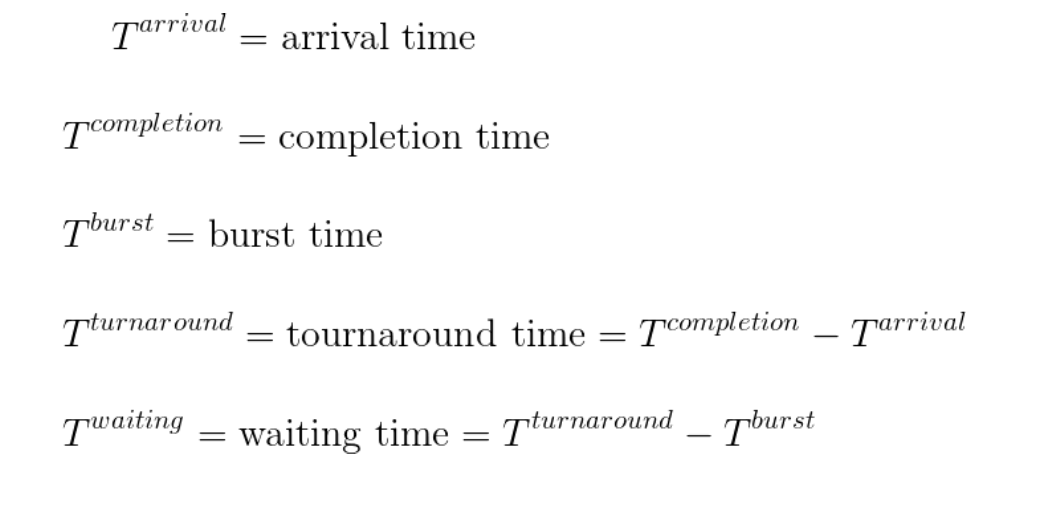
\includegraphics[width=0.7\textwidth,keepaspectratio]{{im/formule}}
        \caption{}    
    \end{center}
    \end{figure}
\subsection{Criteri/metriche di scheduling}
Esistono diversi criteri da considerare quando si tenta di selezionare l'algoritmo di scheduling "migliore", e deve prendere in considerazione:
\begin{itemize}
    \item Utilizzo della CPU, ossia la percentuale di tempo in cui la CPU è occupata
    Idealmente la CPU sarebbe occupata il 100\% del tempo, in modo da sprecare 0 cicli CPU
    Su un sistema reale, l'utilizzo della CPU dovrebbe variare dal 40\% (con carico leggero) al 90\% (con carico pesante)
    \item Throughput, ossia il numero di processi completati in un'unità di tempo. 
    \item Tournaround time, ossia il tempo necessario per il completamento di un particolare processo, dall'invio al completamento. Include tutto il tempo di attesa
    \item Waiting time, ossia il tempo necessario ai processi trascorrono nella coda pronta aspettando il proprio turno per salire sulla CPU. I processi nello stato di attesa non sono sotto il controllo dello scheduler della CPU (semplicemente non sono pronti per essere eseguiti).\footnote{Da non confondere con lo waiting state}
    \item Response time, ossia il tempo impiegato dall'emissione di un comando all'inizio di una risposta a tale comando. Si usa principalmente, per processi interattivi
\end{itemize}

Idealmente, si sceglie uno scheduler della CPU che ottimizzi tutte le metriche contemporaneamente infatti quanto è stado detto sopra è impossibile ed è necessario un compromesso. L'obiettivo era di scegliere un algoritmo di pianificazione in base alla sua capacità di soddisfare una data politica.\\
L'obiettivo dello scheduling è di ridurre al minimo il tempo medio di risposta\footnote{Tipico dei sistemi interattivi}:
\begin{itemize} 
    \item Minimizzare il \textbf{tempo medio} di risposta
        \item Fornire l'output all'utente il più rapidamente possibile
    \item Ridurre al minimo il tempo di risposta massimo
        \item Limite nel caso peggiore
    \item Ridurre al \textbf{minimo} la varianza del tempo di risposta
        \item Gli utenti accettano di più un sistema coerente e prevedibile piuttosto che uno incoerente
\end{itemize}

\pagebreak

Massimizzare il throughput significa\footnote{Tipico dei sistemi batch. I \textbf{sistemi batch} (o "batch processing systems" in inglese) sono un tipo di sistema informatico che esegue una serie di lavori o processi in una sequenza predefinita, senza interazione diretta con l'utente o l'operatore del sistema.
In un sistema batch, i lavori vengono raccolti in un'area di elaborazione chiamata "coda di lavoro" o "batch queue". Il sistema elabora poi i lavori uno per uno, seguendo un ordine predefinito, e può eseguirli in background, senza richiedere l'input dell'utente durante l'esecuzione. Fonte: Wikipedia}:
\begin{itemize}
    \item Riduzione al minimo dell'overhead (cambio di contesto del sistema operativo)
    \item Utilizzo efficiente delle risorse di sistema (CPU e dispositivi I/O)
    \item Ridurre al minimo i tempi di attesa
    \item Dare a ogni processo la stessa quantità di tempo sulla CPU 
    \item Potrebbe aumentare il tempo medio di risposta
\end{itemize}


Per le politiche di scheduling assumiamo che:
\begin{itemize}
    \item Vi è un singolo processo per utente
    \item I processi sono indipendenti tra di loro, dunque non vi è comunicazione 
    \item Ogni processo è costituito da un singolo thread
\end{itemize}

\subsection{Algoritmi di Scheduling}
\subsubsection{First-Come-First-Serve (FCFS)}
Il FCFS ha solo una coda FIFO, lo scheduler esegue i lavori fino al completamento nell'ordine di arrivo ed entra in azione solo quando il lavoro attualmente in esecuzione lo richiede un'operazione di I/O (o termina la sua esecuzione). Un lavoro può continuare a utilizzare la CPU a tempo indeterminato (ovvero fino a quando non si blocca) per questo è di tipo Non-preemptive. 
\pagebreak
\subsubsection*{Esempi}
\begin{enumerate}
    \item Consideriamo la seguente coda di processi: 
    \begin{figure}[hbt]
        \begin{center}
            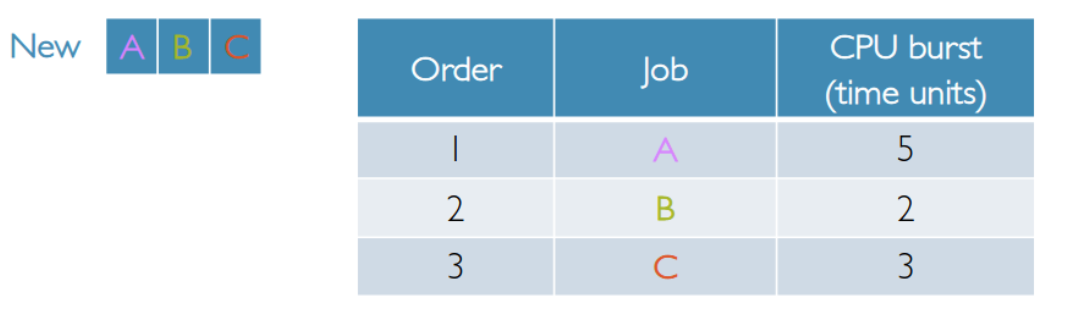
\includegraphics[width=0.7\textwidth,keepaspectratio]{{im/fcfs1}}
            \caption{}    
        \end{center}
    \end{figure}
    \begin{itemize}
        \item I processi vengono creati allo stesso istante, dunque l'arrival time per tutti i processi è l'istante 0. Successivamente, tutti e tre i processi vengono messi nella ready queue
        \begin{figure}[hbt]
            \begin{center}
                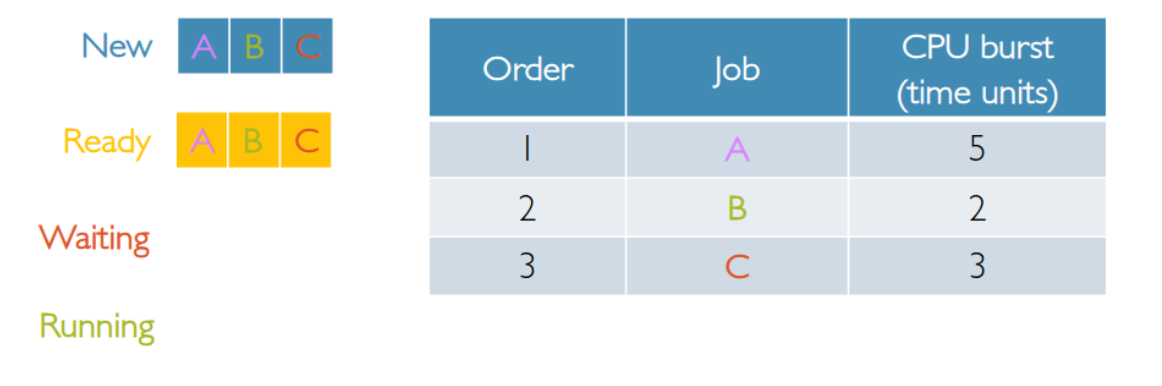
\includegraphics[width=0.7\textwidth,keepaspectratio]{{im/fcfs12}}
                \caption{}    
            \end{center}
        \end{figure}
        \item Di seguito, lo scheduling FCFS seleziona il primo processo della ready queue, ossia il processo A, spostandolo in stato di ready e completando la sua esecuzione
        \begin{figure}[hbt]
            \begin{center}
                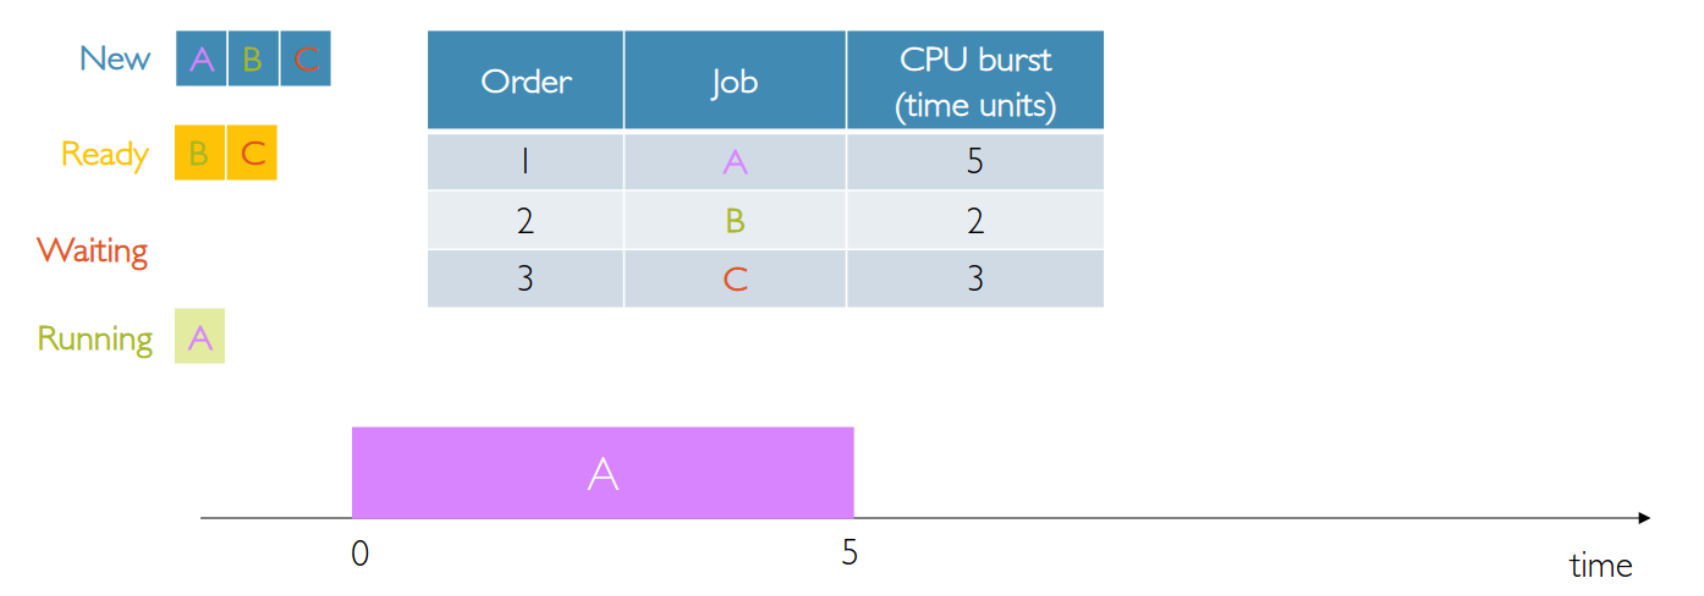
\includegraphics[width=0.7\textwidth,keepaspectratio]{{im/fcfs13}}
                \caption{}    
            \end{center}
        \end{figure}
        \pagebreak
        \item Una volta terminato il processo A, lo scheduler ripeterà le stesse operazioni fino a che tutti i processi non saranno terminati
        \begin{figure}[hbt]
            \begin{center}
                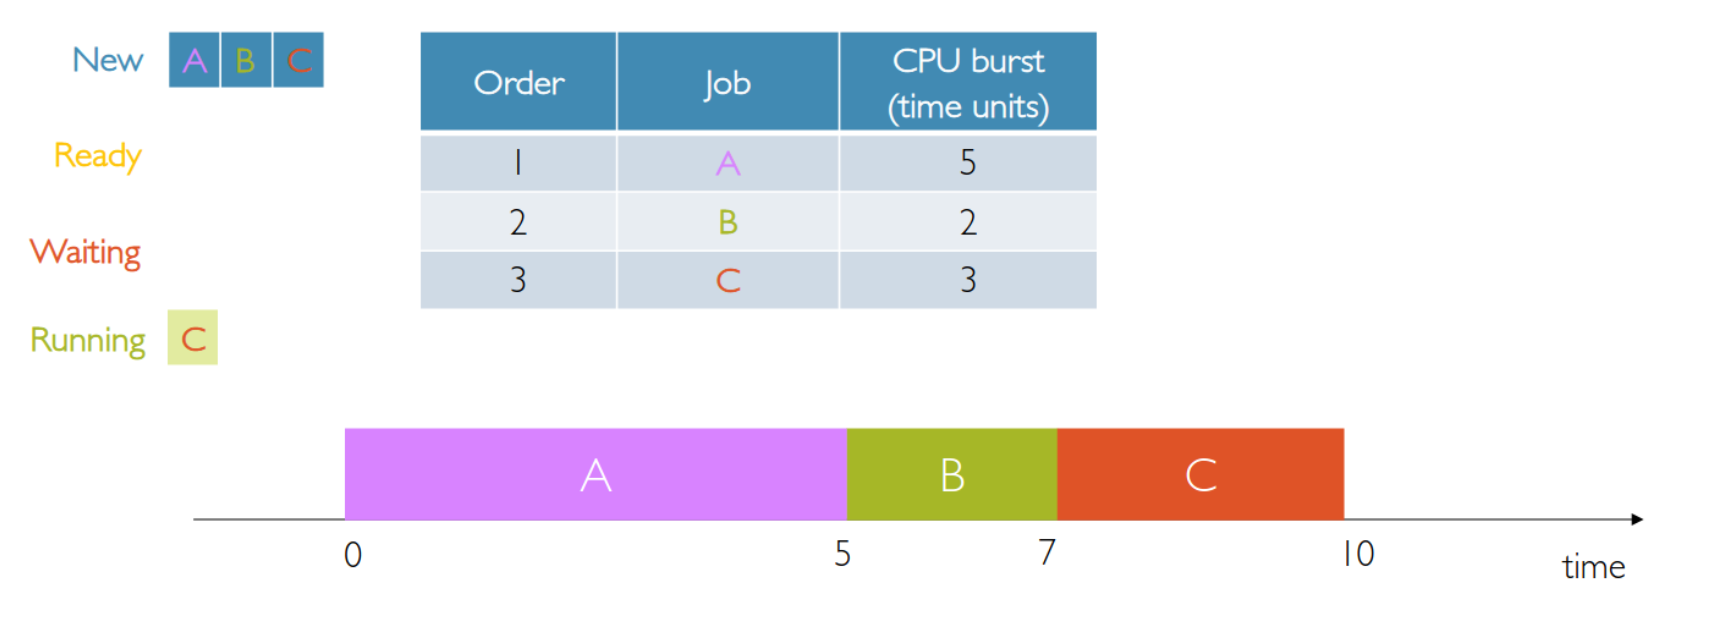
\includegraphics[width=0.7\textwidth,keepaspectratio]{{im/fcfs14}}
                \caption{}    
            \end{center}
        \end{figure}
        \item Una volta terminati tutti i processi, calcoliamo il waiting time medio:
        \begin{itemize}
            \item Per il processo A si ha: \\
            $T_{waiting} = T_{turnaround} - T_{burst} = T_{completion} - T_{arrival} - T_{burst} = 5 - 0 - 5 = 0$
            \item Per il processo B si ha:\\
            $T_{waiting} = T_{turnaround} - T_{burst} = T_{completion} - T_{arrival} - T_{burst} = 7 - 0 - 2 = 5$
            \item Per il processo C si ha:\\
            $T_{waiting} = T_{turnaround} - T_{burst} = T_{completion} - T_{arrival} - T_{burst} = 10 - 0 - 3 = 7$
            \item Il waiting time medio, quindi, sarà:\\
            $\bar{T}_{waiting} = \frac{1}{n}\sum\limits_{i=0}^{n} T_{i}^{waiting}$ = $\frac{0 + 5 + 7}{3} = \frac{12}{3} = 4$
        \end{itemize}
    \end{itemize}
    \item Nel seguente scenario, utilizzando sempre uno scheduling FCFS, si ha:
    \begin{figure}[hbt]
        \begin{center}
            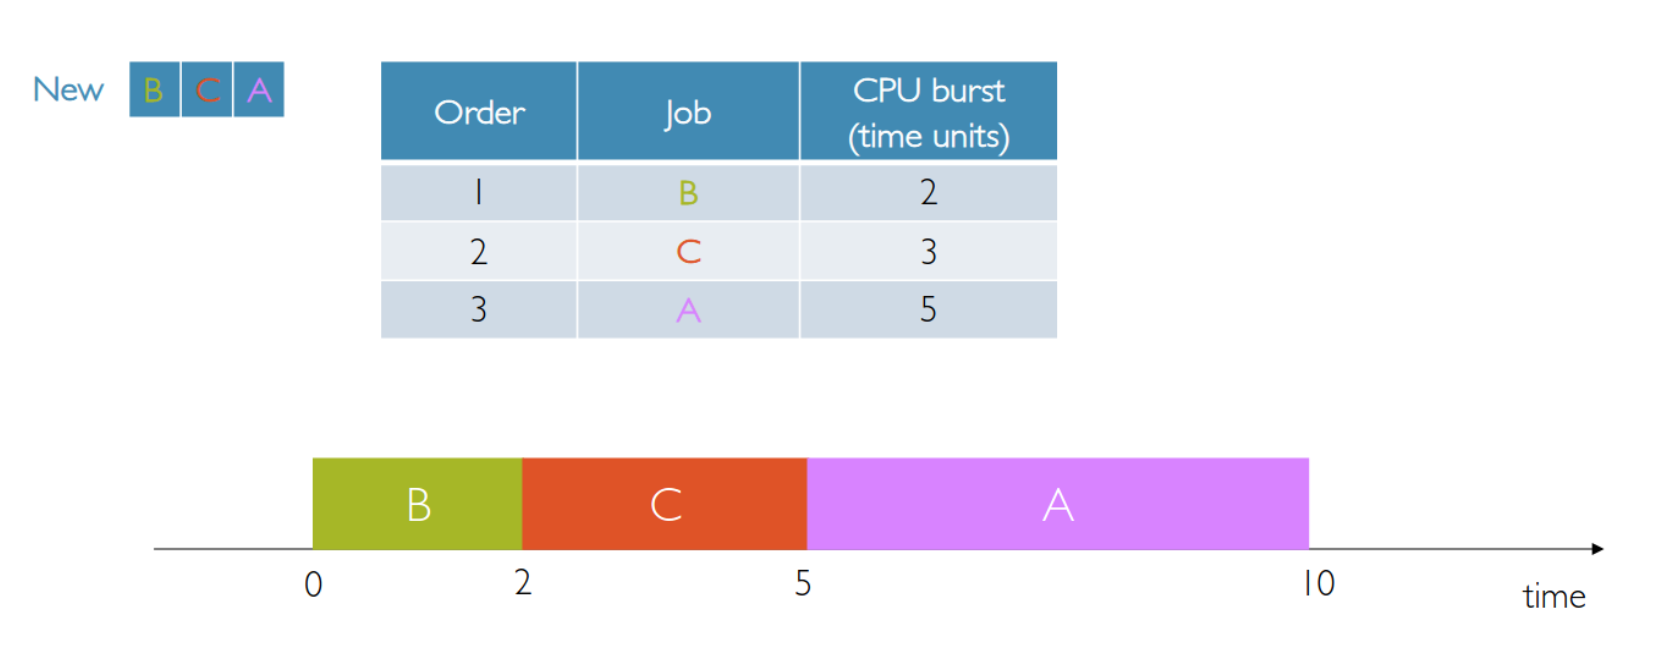
\includegraphics[width=0.7\textwidth,keepaspectratio]{{im/fcfs21}}
            \caption{}    
        \end{center}
    \end{figure}
    \begin{itemize}
        \item Il waiting time medio, quindi, sarà:\\
        $\bar{T}_{waiting} = \frac{1}{n}\sum\limits_{i=0}^{n} T_{i}^{waiting}$ = $\frac{0 + 5 + 2}{3} = \frac{7}{3} \simeq 2.3$
    \end{itemize}
\pagebreak
    \item Consideriamo il seguente scenario:
    \begin{figure}[hbt]
        \begin{center}
            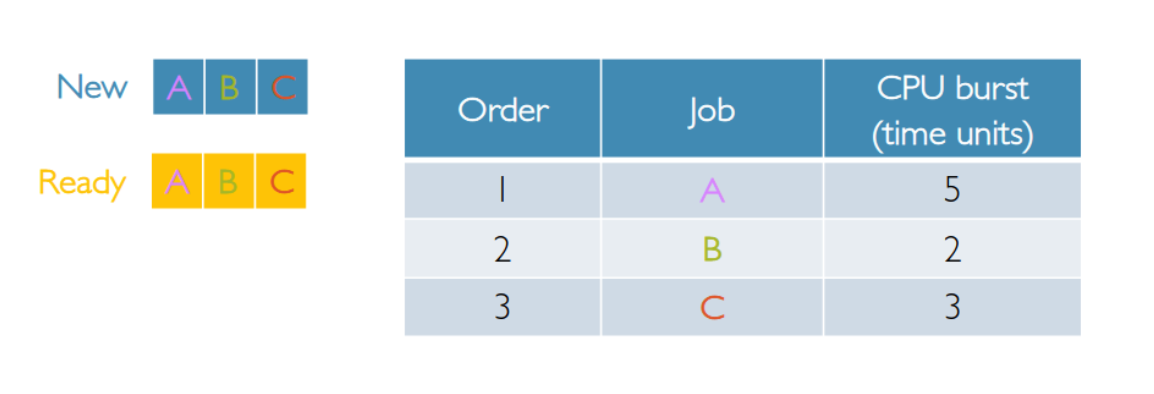
\includegraphics[width=0.7\textwidth,keepaspectratio]{{im/fcfs31}}
            \caption{}    
        \end{center}
    \end{figure}
    
    \begin{itemize}
        \item Supponiamo che dopo 2 unità temporali il processo A esegua una richiesta I/O, entrando quindi in stato di waiting, la quale verrà completata dopo un istante.
        Attenzione: poiché il tempo in attesa I/O non viene calcolato nel waititng time, sarà necessario sottrarre un istante dal waiting time del processo A.
        \begin{figure}[hbt]
            \begin{center}
                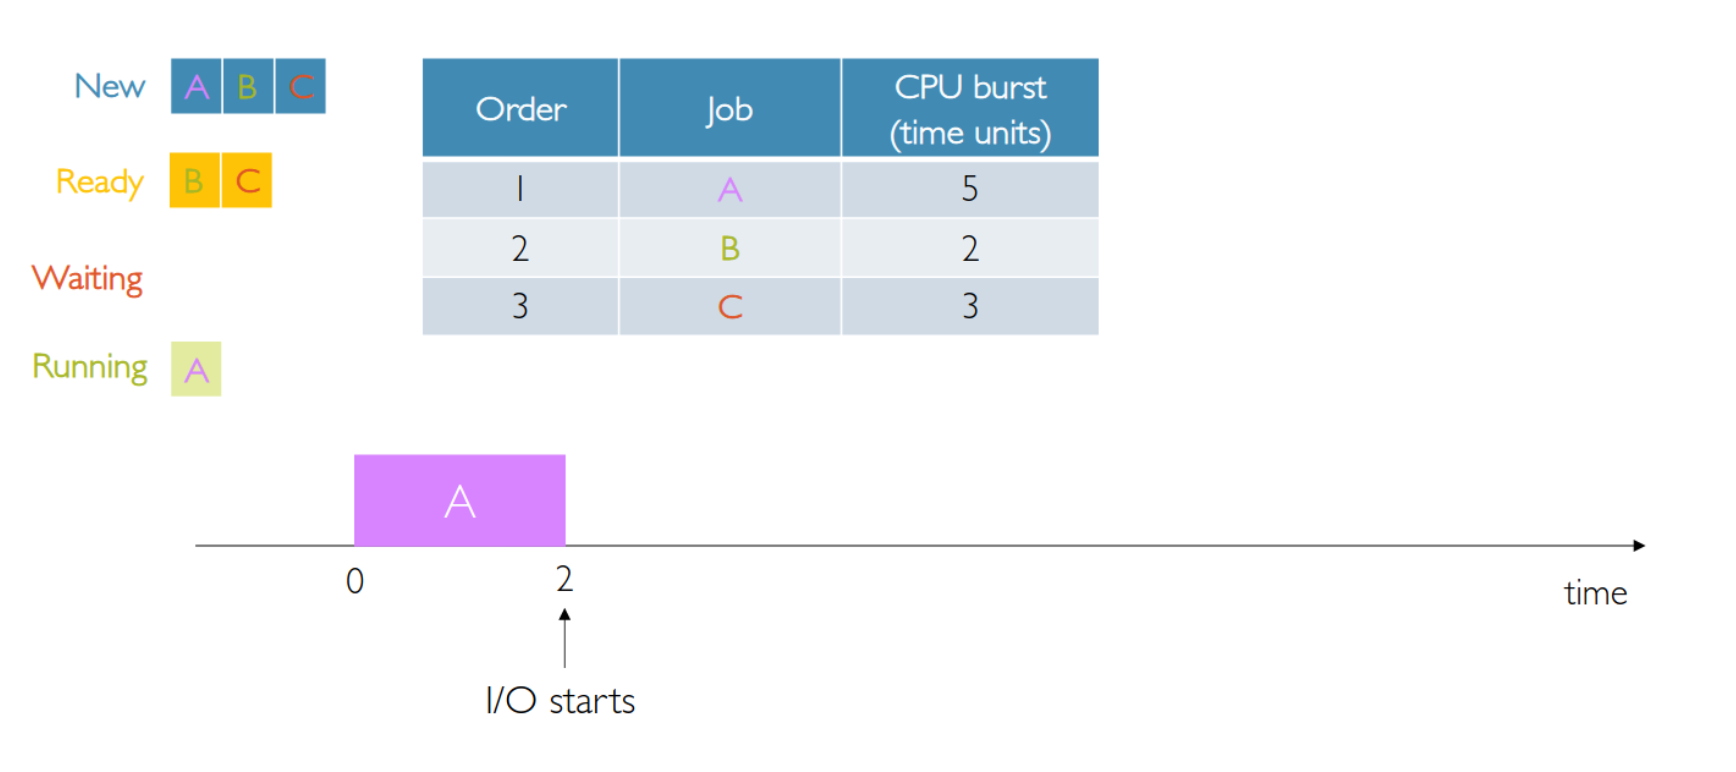
\includegraphics[width=0.7\textwidth,keepaspectratio]{{im/fcfs32}}
                \caption{}    
            \end{center}
        \end{figure}
        \item Una volta entrato in stato di waiting, lo scheduler selezionerà il processo seguente nella coda, ossia il processo B, portandolo a termine
        \begin{figure}[hbt]
            \begin{center}
                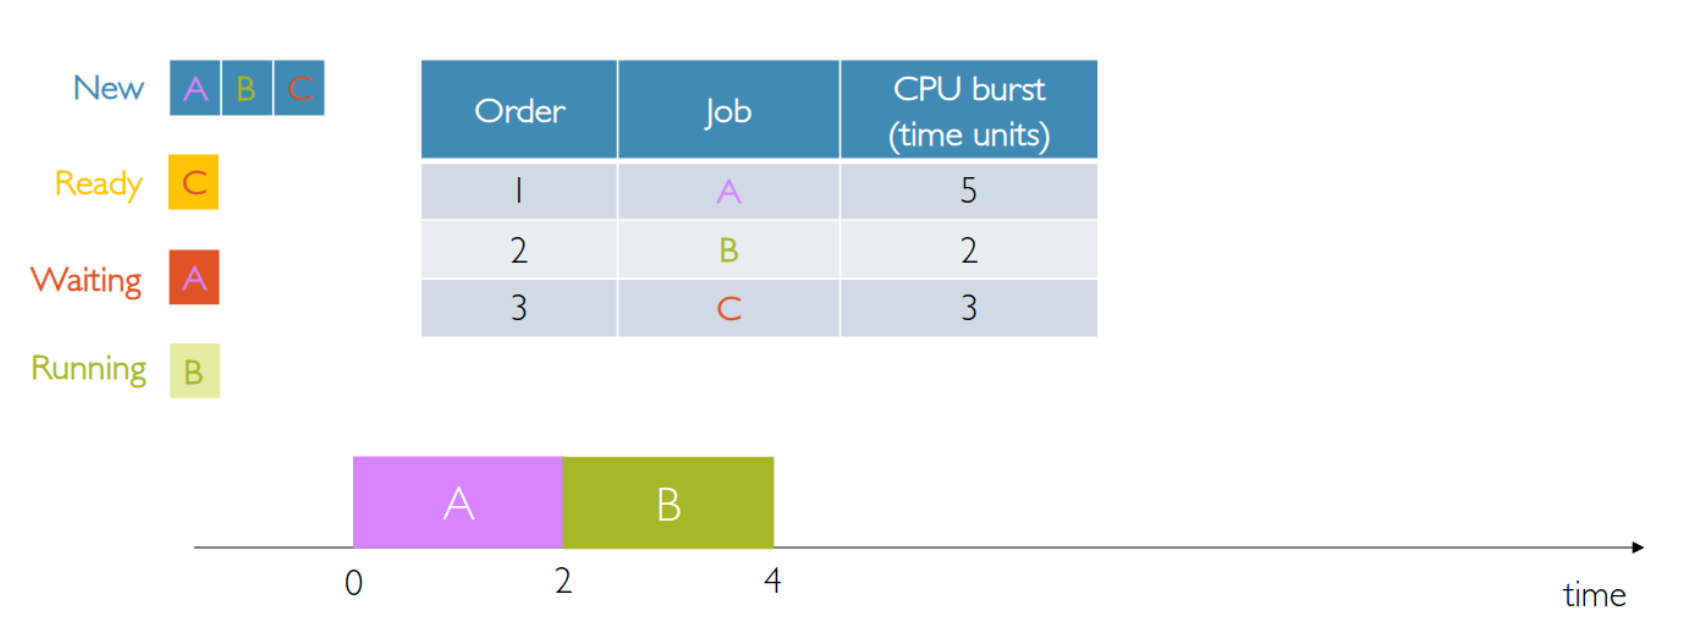
\includegraphics[width=0.7\textwidth,keepaspectratio]{{im/fcfs33}}
                \caption{}    
            \end{center}
        \end{figure}
        \pagebreak
        \item Una volta terminata l'esecuzione del processo B, il processo A verrà selezionato per riprendere l'esecuzione.
        Attenzione: viene selezionato il processo A e non il processo C poiché l'algo- ritmo FCFS utilizza una queue basata sull'arrival time dei processi
        \begin{figure}[hbt]
            \begin{center}
                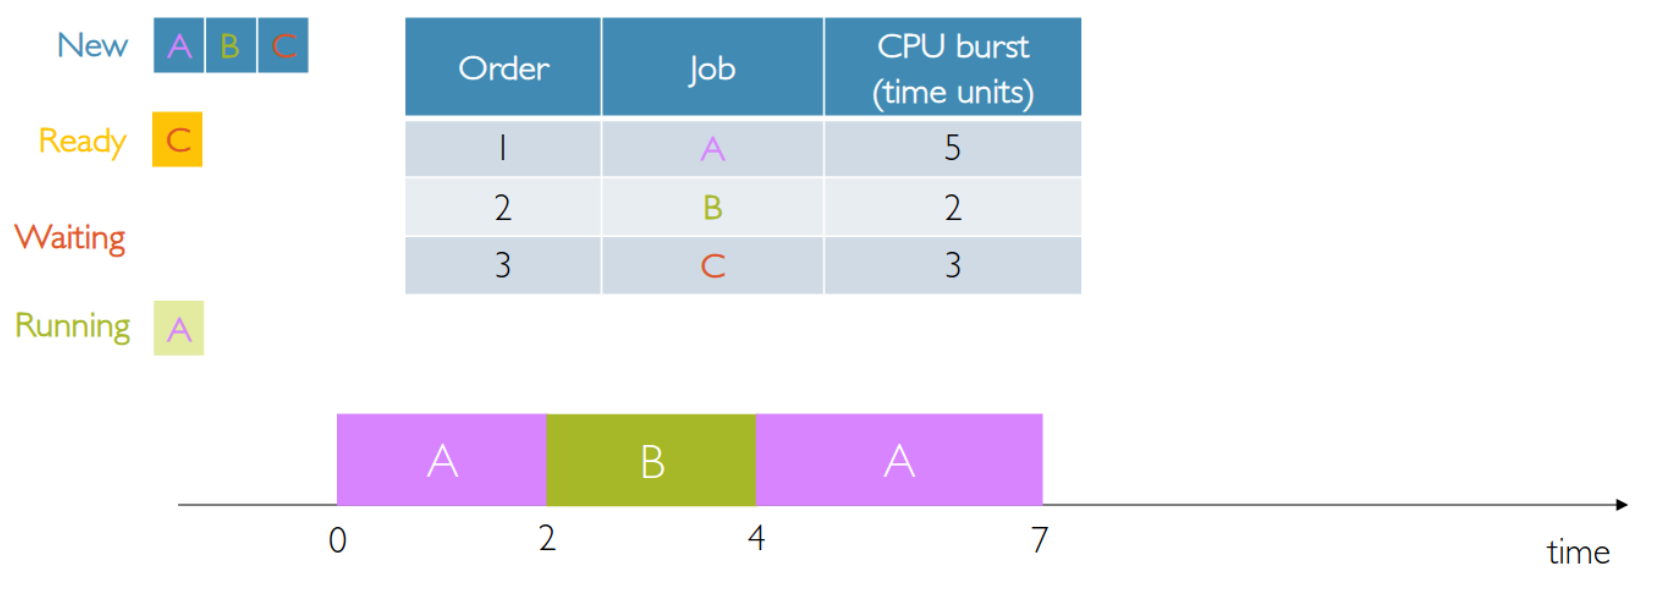
\includegraphics[width=0.7\textwidth,keepaspectratio]{{im/fcfs34}}
                \caption{}    
            \end{center}
        \end{figure}
        \item Infine, il waiting time medio sarà:
        \begin{figure}[hbt]
            \begin{center}
                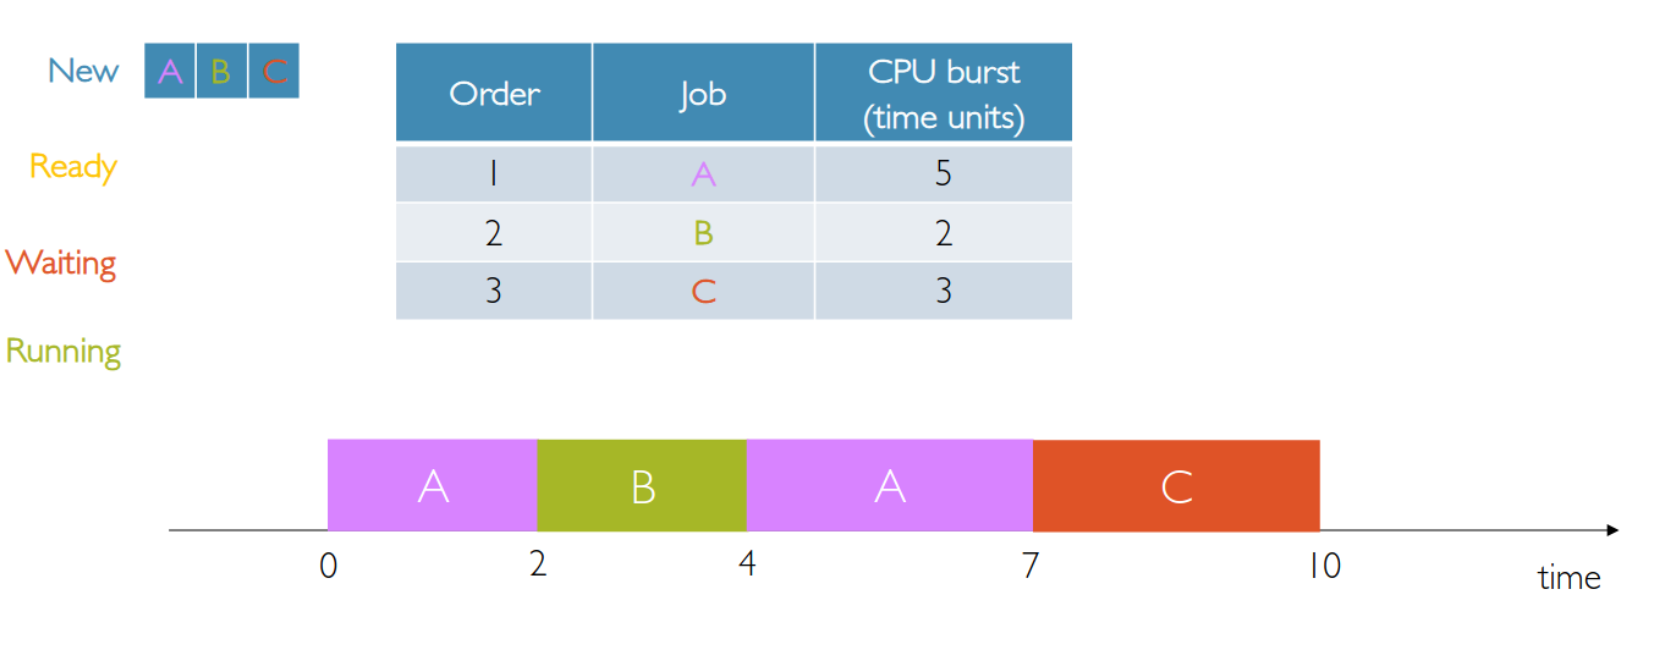
\includegraphics[width=0.7\textwidth,keepaspectratio]{{im/fcfs35}}
                \caption{}    
            \end{center}
        \end{figure}
        \\
        $\bar{T}_{waiting} = \frac{1}{n}\sum\limits_{i=0}^{n} T_{i}^{waiting}$ = $\frac{1 + 2 + 7}{3} = \frac{10}{3} \simeq 3.3$
    \end{itemize}
\end{enumerate}
\subsubsection*{Pro e Contro}
Uno dei \textbf{vantaggi} è la semplicità di implementazione.\\
Tra gli \textbf{svantaggi}:
\begin{itemize} 
    \item Il tempo di attesa (medio) è molto variabile in quanto i lavori di breve durata della CPU possono rimanere indietro quelli molto lunghi.
    \item effetto convoglio: scarsa sovrapposizione tra CPU e I/O poiché i lavori legati alla CPU costringeranno i lavori legati all'I/O ad attendere.
\end{itemize}
\pagebreak
\subsubsection{Round - Robin (RR)}

Il Round Robin è un algoritmo di scheduling \textbf{preemptive} dove viene selezionato il primo processo presente in ready queue dove i burst della CPU sono assegnati con limiti chiamati \textbf{time quantum} o \textbf{(time slice)}. 

\begin{figure}[hbt]
    \begin{center}
        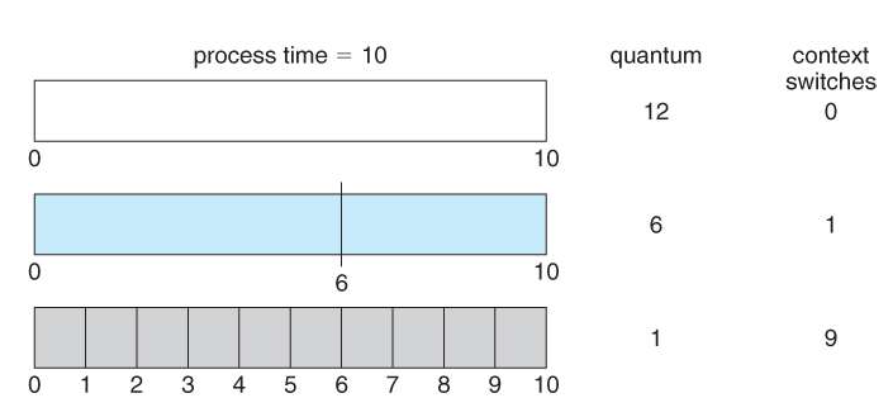
\includegraphics[width=0.5\textwidth,keepaspectratio]{{im/timeslice}}
        \caption{}    
    \end{center}
\end{figure} 

Quando un lavoro viene assegnato alla CPU, viene impostato un timer per un determinato valore, se il lavoro termina prima della scadenza del quanto temporale, viene sostituito da CPU proprio come il normale algoritmo FCFS. Se il timer si spegne per primo, il lavoro viene scambiato fuori dalla CPU e spostato nel back-end della coda dei pronti.\\
Viene utilizzato in molti sistemi di time-sharing in combinazione con gli interrupt del timer. \\
La queue pronta viene mantenuta come queue circolare. Quando tutti i lavori hanno avuto un turno, lo scheduler ne assegna un altro al primo lavoro girare e così via. L'algoritmo RR viene considerato equo in quanto condivide la CPU equamente tra tutti i lavori. Il tempo medio di attesa può essere più lungo rispetto ad altri algoritmi di scheduling.\\
Il limite superiore per lo start time di un processo in una coda di n processi utilizzando uno scheduler RR corrisponde a $sup\{T_{i}^{start}\}$ = $\delta$ · (i - 1), dove i $\in$ $[1,n]$ e dove $\delta$ è il time slice.

\subsubsection*{Esempi}
\begin{itemize}
    \item Consideriamo la seguente coda dei processi utilizzando un algoritmo RR con un time slice di 2 e un context switch trascurabile:
    \begin{figure}[hbt]
        \begin{center}
            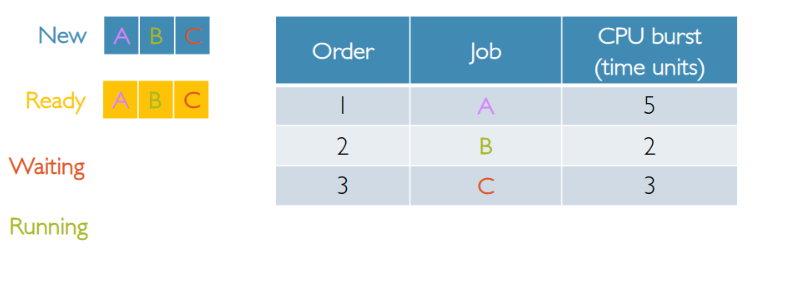
\includegraphics[width=0.5\textwidth,keepaspectratio]{{im/rr1}}
            \caption{}    
        \end{center}
    \end{figure}
    \item Il primo processo a prendere il controllo della CPU è il processo A, venendo bloccato ed aggiunto alla ready queue dopo 2 unità temporali per via del time slice
    \begin{figure}[hbt]
        \begin{center}
            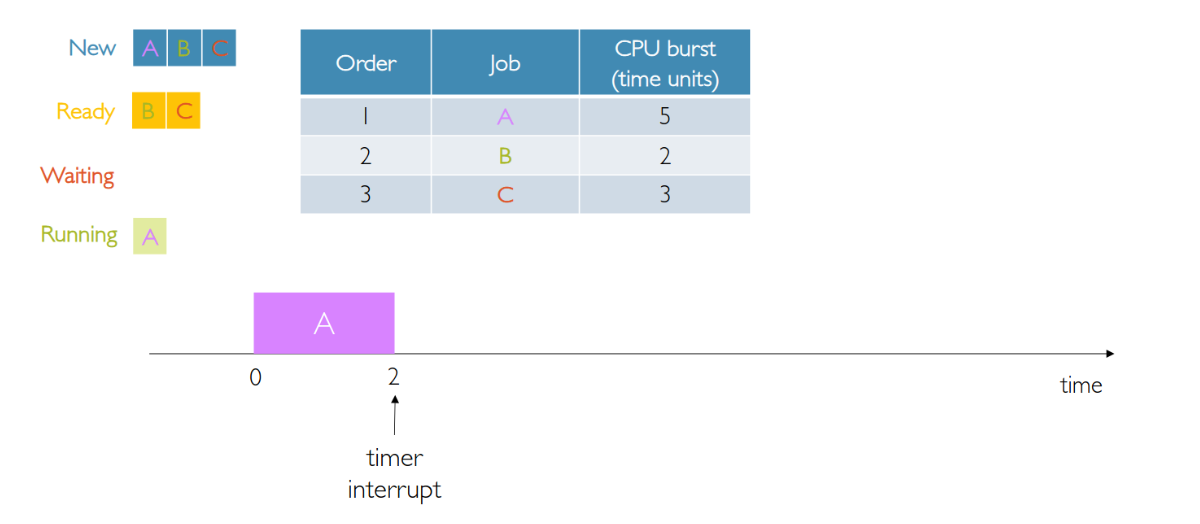
\includegraphics[width=0.5\textwidth,keepaspectratio]{{im/rr12}}
            \caption{}    
        \end{center}
    \end{figure}
    \pagebreak
    \item Successivamente, il processo B prende controllo della CPU, venendo anch'esso bloc- cato dopo 2 unità temporali. In questo caso, tuttavia, il processo B non verrà aggiunto alla fine della ready queue poiché la sua esecuzione è terminata
    \begin{figure}[hbt]
        \begin{center}
            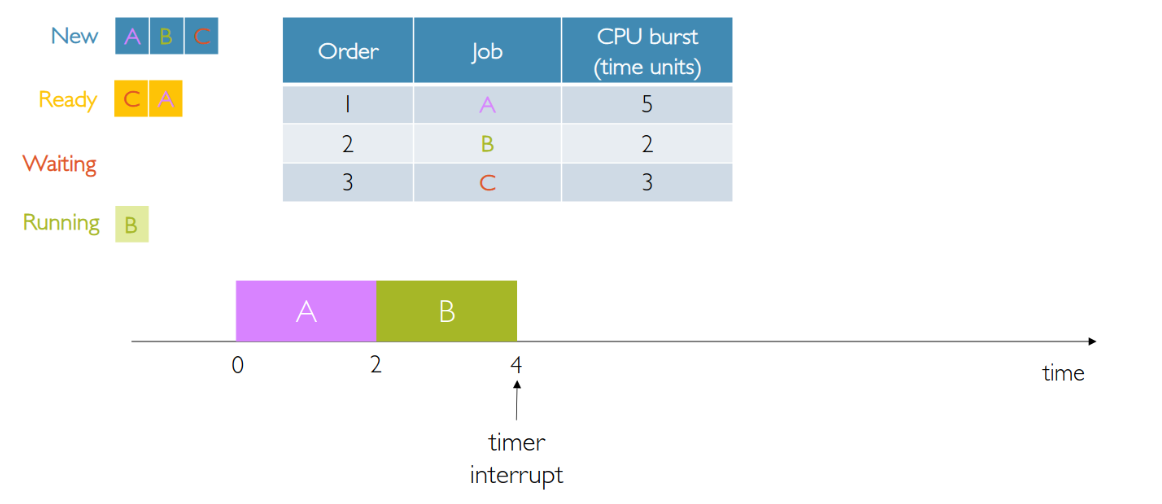
\includegraphics[width=0.5\textwidth,keepaspectratio]{{im/rr13}}
            \caption{}    
        \end{center}
    \end{figure}
    \item Di seguito, il processo C prenderà il controllo, venendo bloccato dopo 2 tempi
    \begin{figure}[hbt]
        \begin{center}
            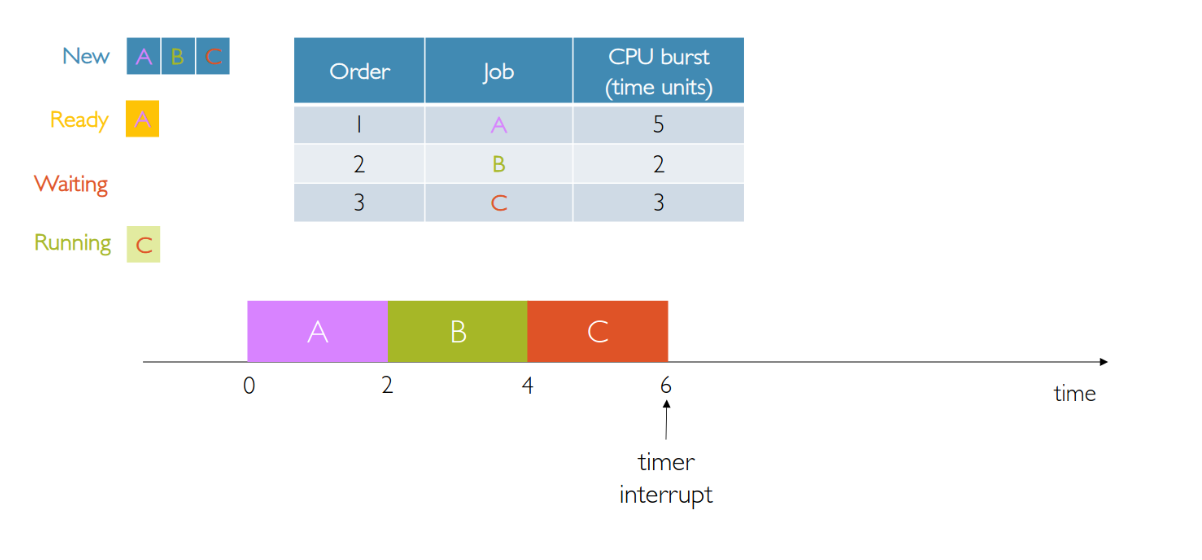
\includegraphics[width=0.5\textwidth,keepaspectratio]{{im/rr14}}
            \caption{}    
        \end{center}
    \end{figure}
    \item Infine, vengono eseguiti i processi A e C finché essi non verranno completati
    \begin{figure}[hbt]
        \begin{center}
            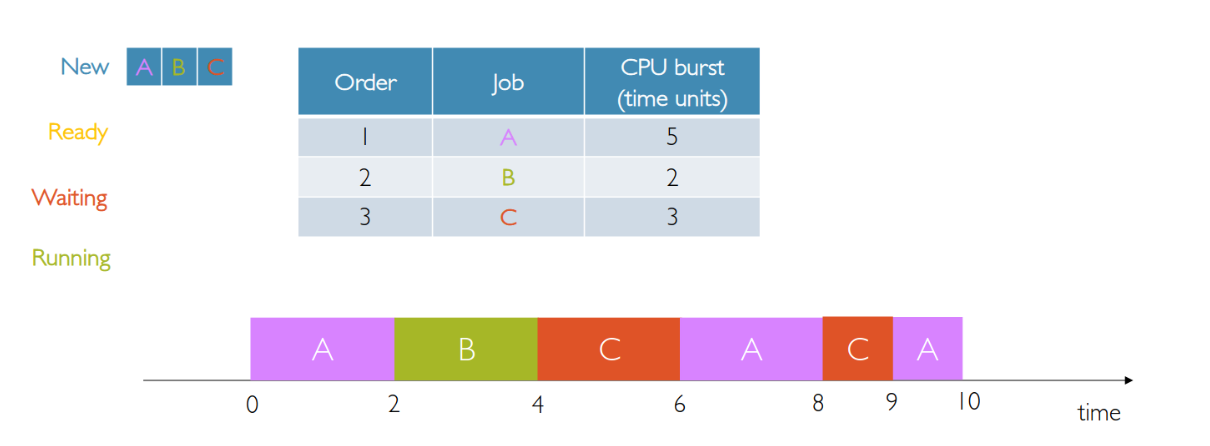
\includegraphics[width=0.5\textwidth,keepaspectratio]{{im/rr15}}
            \caption{}    
        \end{center}
    \end{figure} 
    \item Il waiting time medio, quindi, sarà:\\

    $\bar{T}_{waiting} = \frac{1}{n}\sum\limits_{i=0}^{n} T_{i}^{waiting}$ = $\frac{5 + 2 + 6}{3} = \frac{13}{3} \simeq 4.3$
\end{itemize}
\pagebreak
\subsubsection{FCFS vs RR}
Confrontando il tournaround time e il waiting time medio tra uno scheduler FCFS e uno scheduler RR, il primo sembra essere a primo occhio più performante del secondo. \par
Tuttavia, considerando la varianza tra i waiting time di ogni processo, notiamo come il RR risulta essere più equo, fornendo ad ogni processo la stessa quantità di tempo di utilizzo della CPU.
\begin{figure}[hbt]
    \begin{center}
        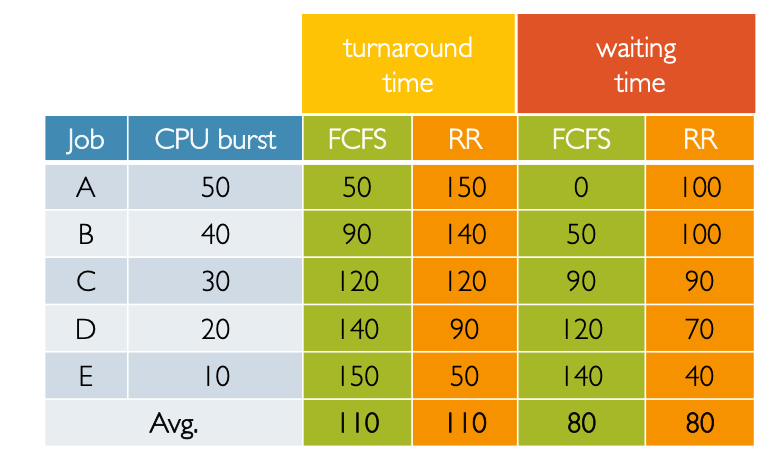
\includegraphics[width=0.5\textwidth,keepaspectratio]{{im/fcfsrr}}
        \caption{}    
    \end{center}
\end{figure} 

\pagebreak

\subsubsection{Shortest-Job-First (SJF)}
Il Shortest-Job-First è u altro algoritmo di scheduling di tipo \textbf{non preemptive} che parte dal presupposto che i tempi di esecuzione siano conosciuti in anticipo. Lo scheduler preleva per primo il lavoro più breve (da qui il nome \textbf{shortest job first}). \par
Una versione \textbf{preemptive} dell'algoritmo shortest job first è l'algoritmo shortest remaining time first dove ogni volta che un nuovo job arriva nella ready queue e il suo CPU burst stimato è minore di quello rimanente del job attualmente in esecuzione, tale job prende controllo della CPU.\par
Lo SJF presenta dei vantaggi infatti risulta ottimale quando l'obiettivo è minimizzare il tempo medio di attesa. Funziona sia con schedulatori preventivi che non preventivi.\par
Tra gli svantaggi possiamo affermare che risulta quasi impossibile prevedere la quantità di tempo CPU di un lavoro. Anche i lavori legati alla CPU a esecuzione prolungata possono morire di \textit{starve} (come hanno fatto implicitamente quelli legati all'I/O priorità maggiore rispetto a loro).\par
Per stimare la lunghezza del prossimo CPU burst, viene utilizzato l'exponential smoothing:
\begin{itemize}
    \item Sia $x_{t}$ la lunghezza effettiva del t-esimo CPU burst
    \item Sia $S_{t+1}$ la lunghezza stimata del $(t + 1)$-esimo CPU burst 
    \item Sia $\alpha$ $\in$ $R$ dove 0 $\geq \alpha \leq$ 1
    \item Si ha che:
    \begin{center}
        $s_{1}$ = $x_{0}$\\
        $s_{t+1} = \alpha x_{t} +(1 - \alpha) s_{t}$
    \end{center}
\end{itemize}

\subsubsection*{Esempi}
\begin{enumerate}
    \item Consideriamo la seguente coda di processi gestita da uno scheduler SJF non preemptive. In tal caso, si ha che:\\
        \begin{figure}[hbt]
            \begin{center}
                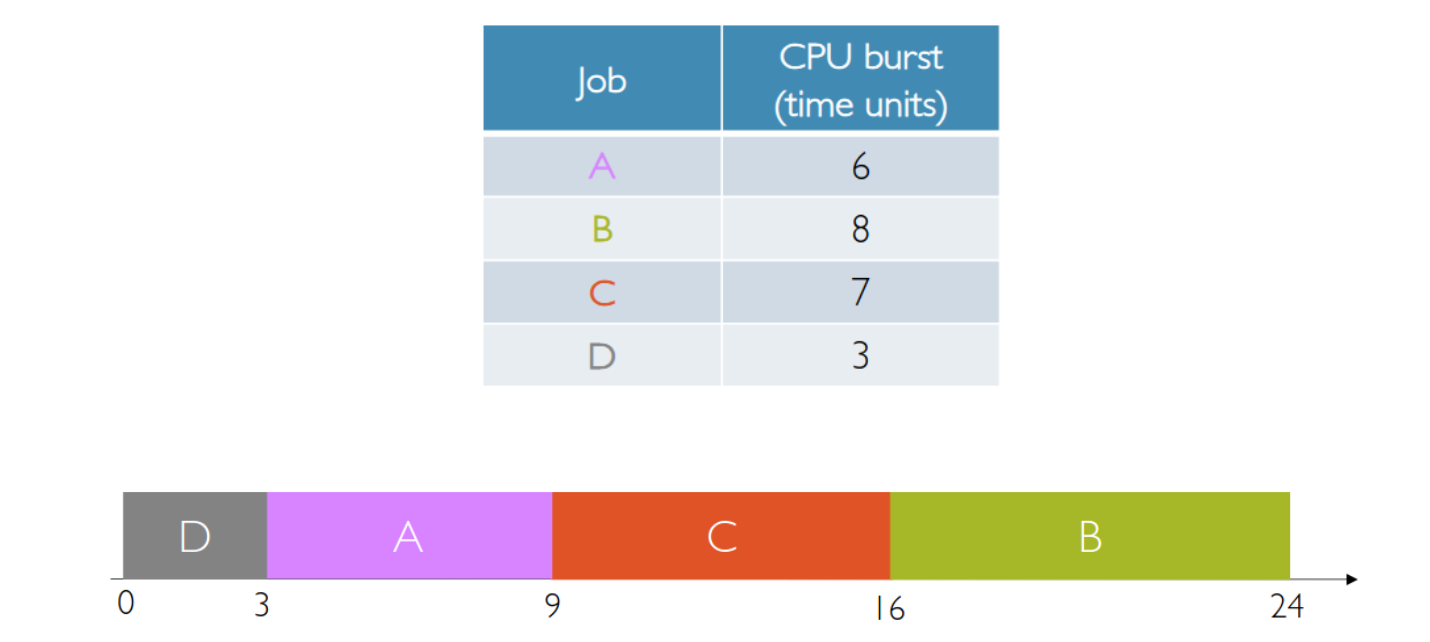
\includegraphics[width=0.5\textwidth,keepaspectratio]{{im/sjf1}}
                \caption{}    
            \end{center}
        \end{figure} \\
        \begin{center}
            $\bar{T}_{ave.waiting}$ = $\frac{3 + 16 + 9 + 0}{4}$ = $\frac{28}{4} = 7$
        \end{center}
    \item Consideriamo la seguente coda di processi gestita da uno scheduler SJF preemptive, ossia uno scheduler SRTF.
    \begin{itemize}
        \item \begin{figure}[hbt]
            \begin{center}
                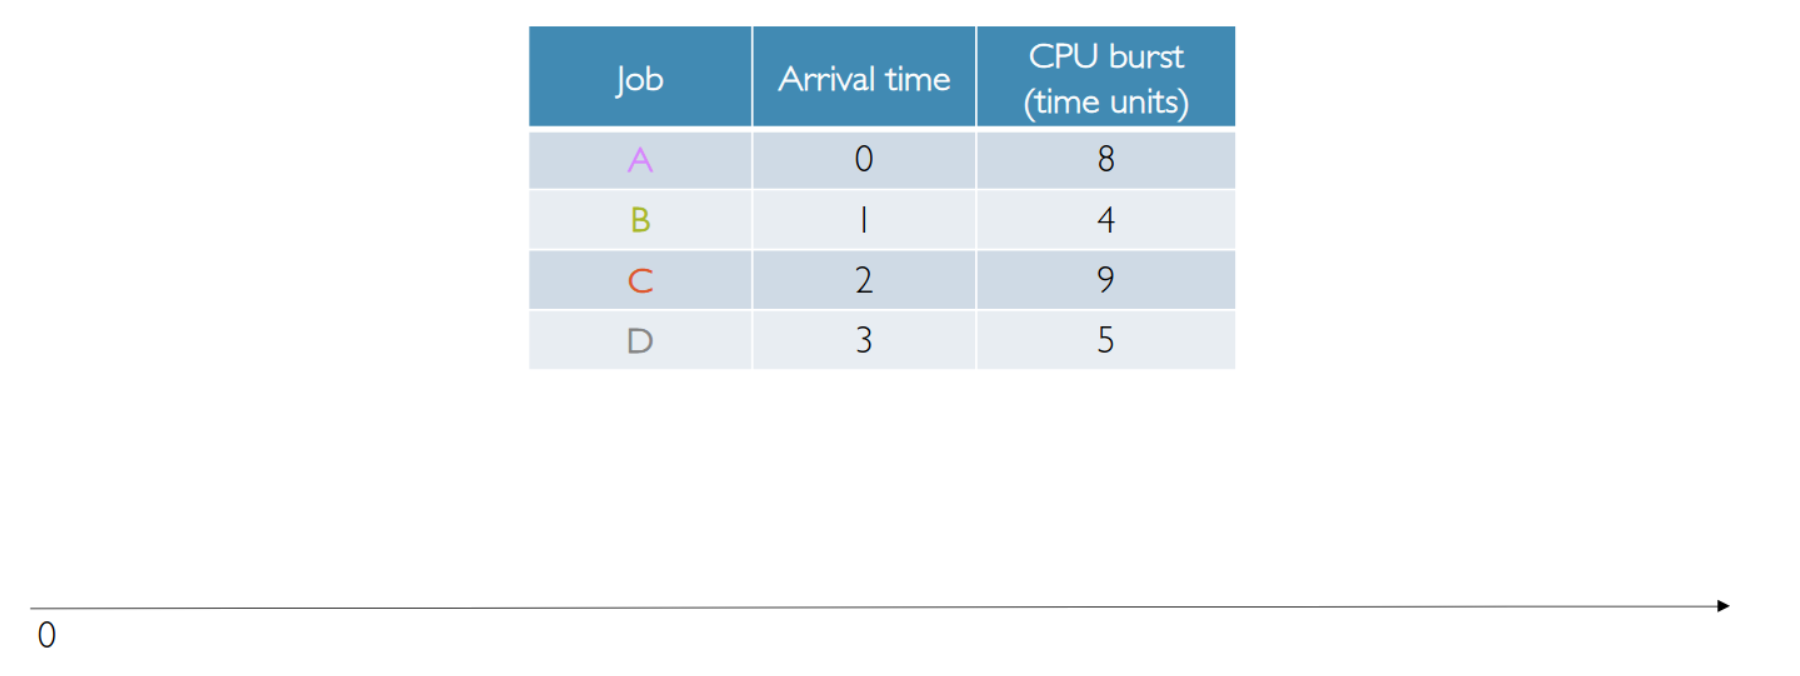
\includegraphics[width=0.5\textwidth,keepaspectratio]{{im/sjf2}}
                \caption{}    
            \end{center}
        \end{figure} 
        \item Il primo job ad essere eseguito è il processo A, poiché il primo ad essere creato ed inserito nella ready queue.
        \begin{figure}[hbt]
            \begin{center}
                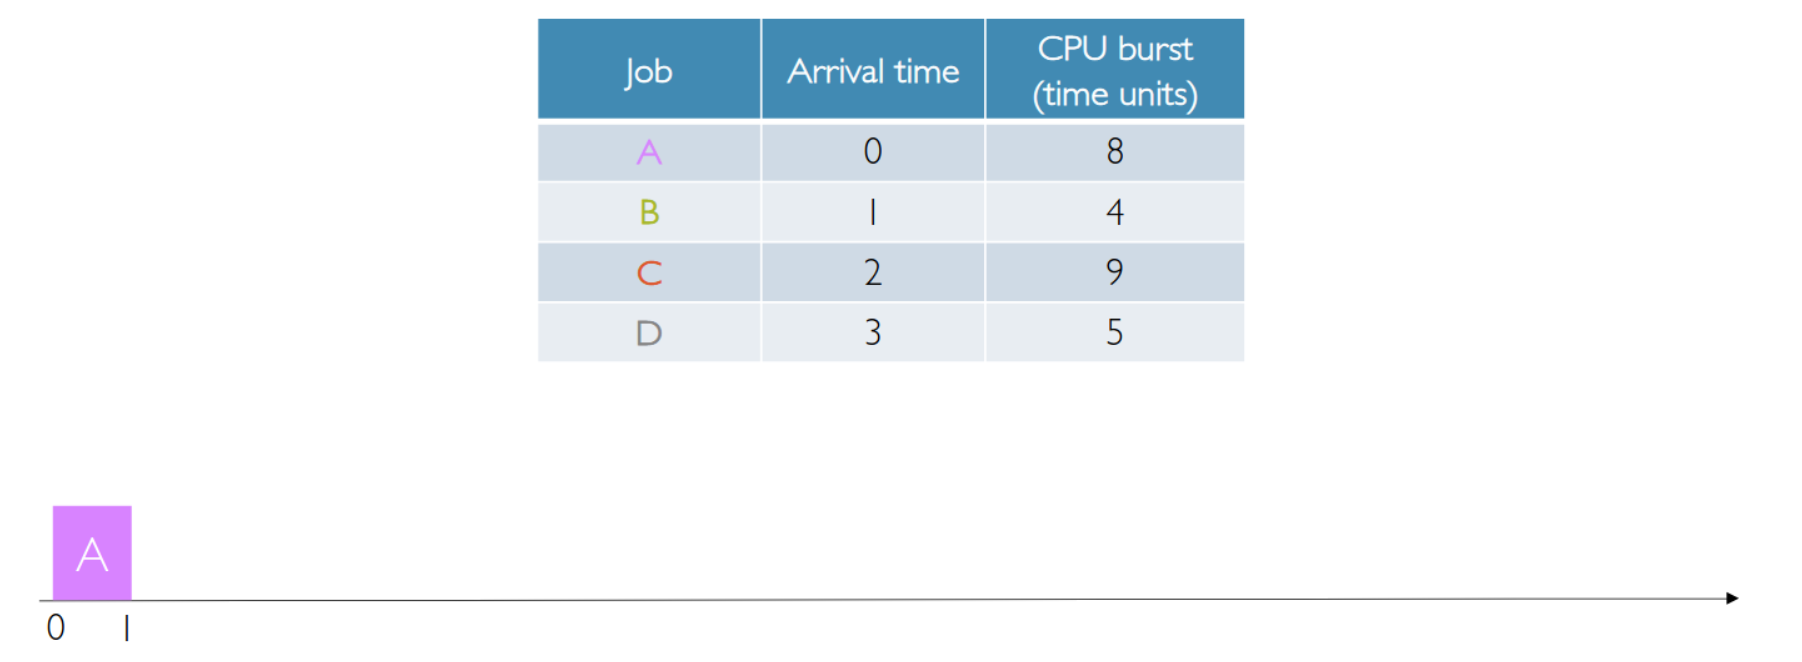
\includegraphics[width=0.5\textwidth,keepaspectratio]{{im/sjf21}}
                \caption{}    
            \end{center}
        \end{figure} 
        \item Una volta che il processo B viene creato, il suo CPU burst stimato, ossia 4, viene comparato con il CPU burst rimanente del processo A, ossia 7. Poiché 4 < 7, allora il processo B prende controllo della CPU.
        Analogamente, nell'istante in cui il processo C viene creato, il suo CPU burst stimato, ossia 9, viene comparato con quello rimanente del processo A, ossia 6, e quello del processo B, ossia 3. Siccome 3 < 7 < 9, allora il processo B mantiene il controllo della CPU.
        Lo stesso ragionamento viene effettuato anche dopo la creazione del processo D, dove il processo B mantiene il controllo (2 < 7 < 5 < 9). Di conseguenza, il processo B verrà eseguito fino al suo completamento.
        \begin{figure}[hbt]
            \begin{center}
                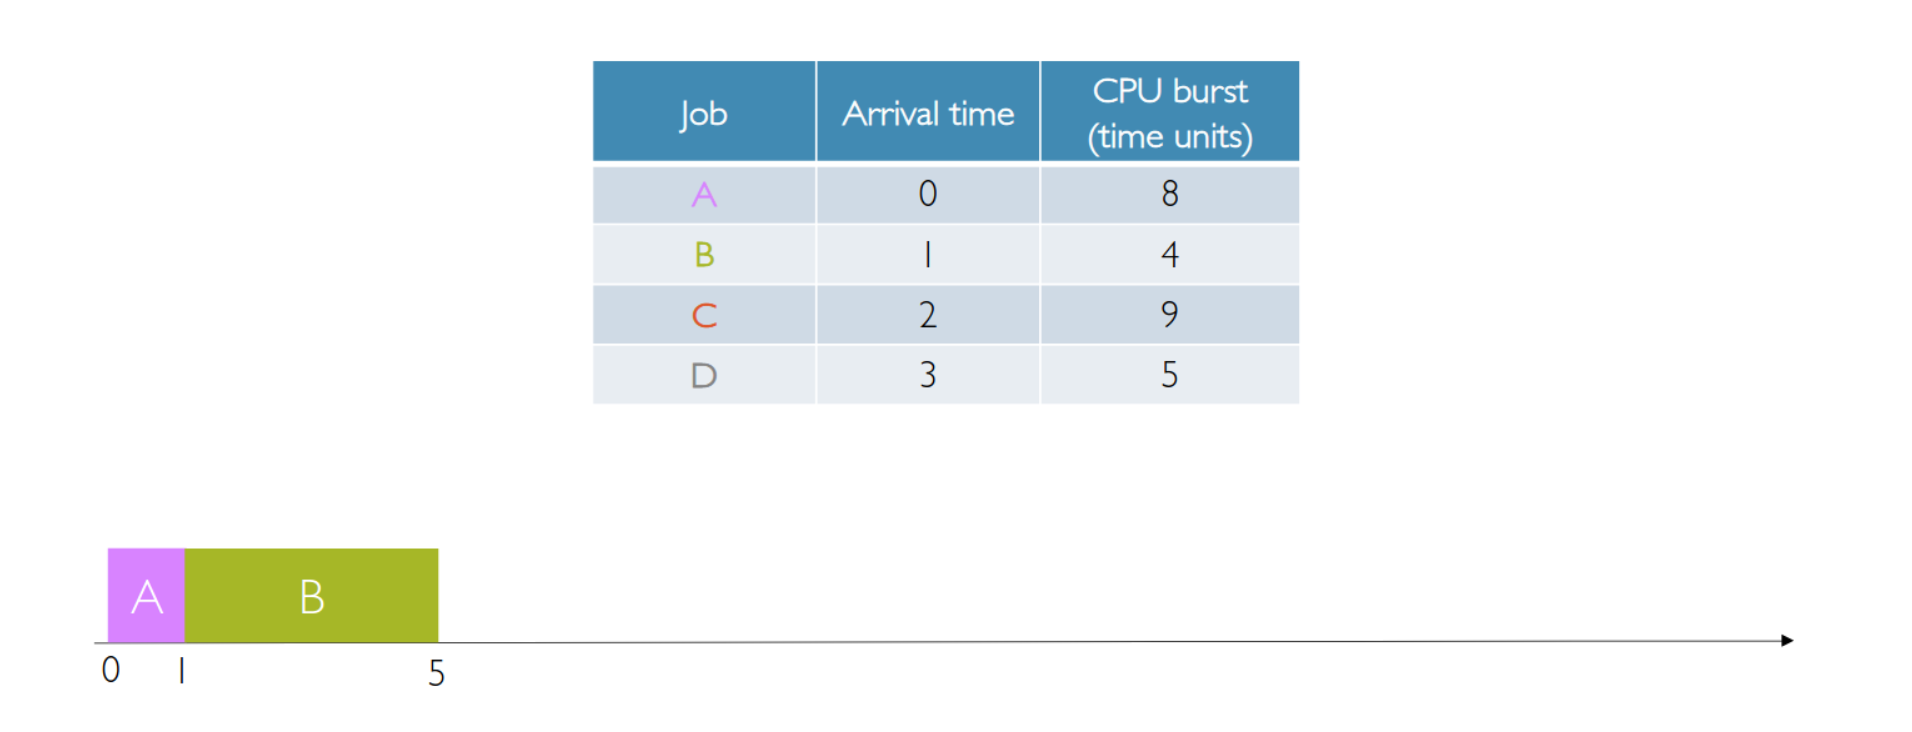
\includegraphics[width=0.5\textwidth,keepaspectratio]{{im/sjf22}}
                \caption{}    
            \end{center}
        \end{figure} 
        \item Una volta completato il processo B, verrà eseguito il processo avente il CPU burst stimato minore:
        \begin{itemize}
            \item  Il processo A ha un CPU burst rimanente pari a 7 
            \item Il processo C ha un CPU burst rimanente pari a 9 
            \item Il processo D ha un CPU burst rimanente pari a 5
            Di conseguenza, verrà eseguito il processo D fino al suo completamento
        \end{itemize}
        \begin{figure}[hbt]
            \begin{center}
                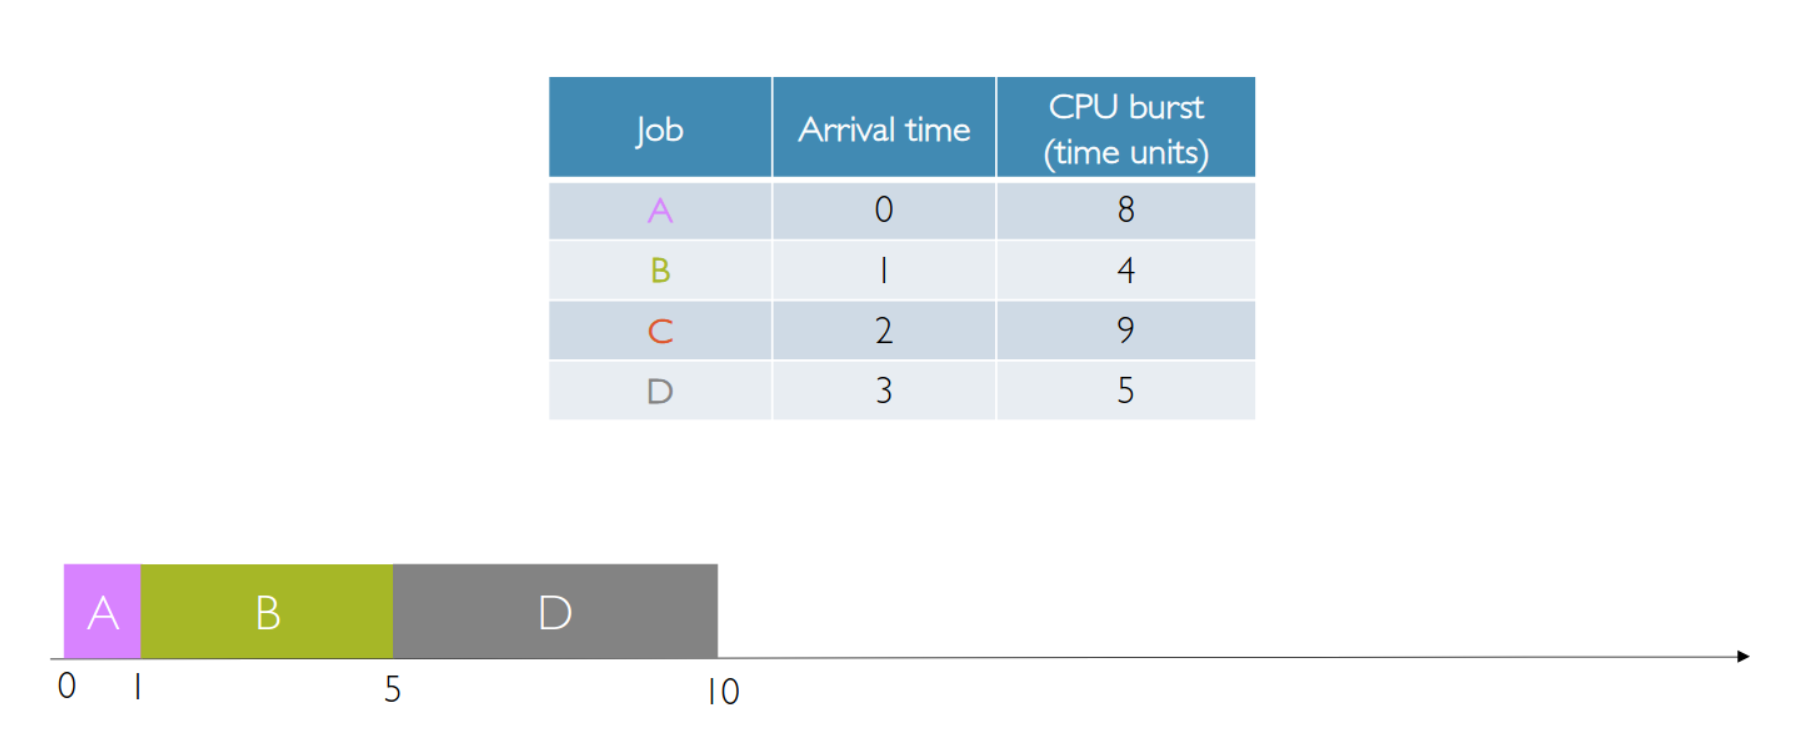
\includegraphics[width=0.5\textwidth,keepaspectratio]{{im/sjf23}}
                \caption{}    
            \end{center}
        \end{figure} 
        \pagebreak
        \item Analogamente al processo D, verranno eseguiti il processo A e il processo C, ognuno di essi fino al loro completamento (poiché, nel frattempo, nessun altro processo viene inserito nella ready queue, dunque non viene mai attivato l'algoritmo di scheduling).
        \begin{figure}[hbt]
            \begin{center}
                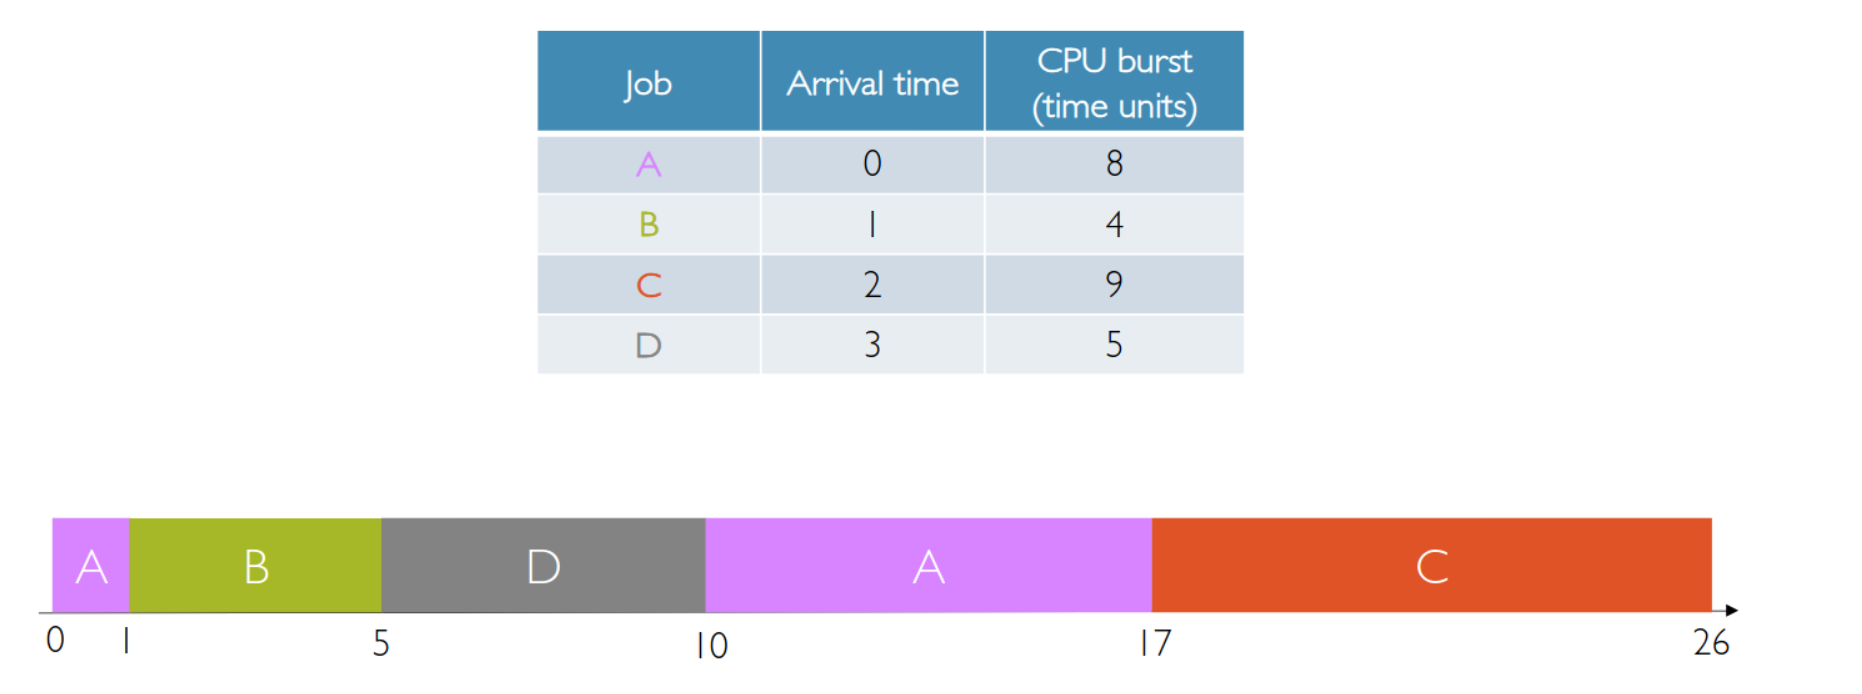
\includegraphics[width=0.5\textwidth,keepaspectratio]{{im/sjf24}}
                \caption{}    
            \end{center}
        \end{figure}
        \begin{center}
            
        $\bar{T}_{ave.waiting}$ = $\frac{(17 - 0 - 8)+(5 - 1 - 4)+(26 - 2 - 9)+(10 - 3 - 5)}{4}$ = $6.5$
    \end{center}
    \end{itemize}
\end{enumerate}

\subsubsection{Confronto tra FCFS, RR e SJF}

\begin{figure}[hbt]
    \begin{center}
        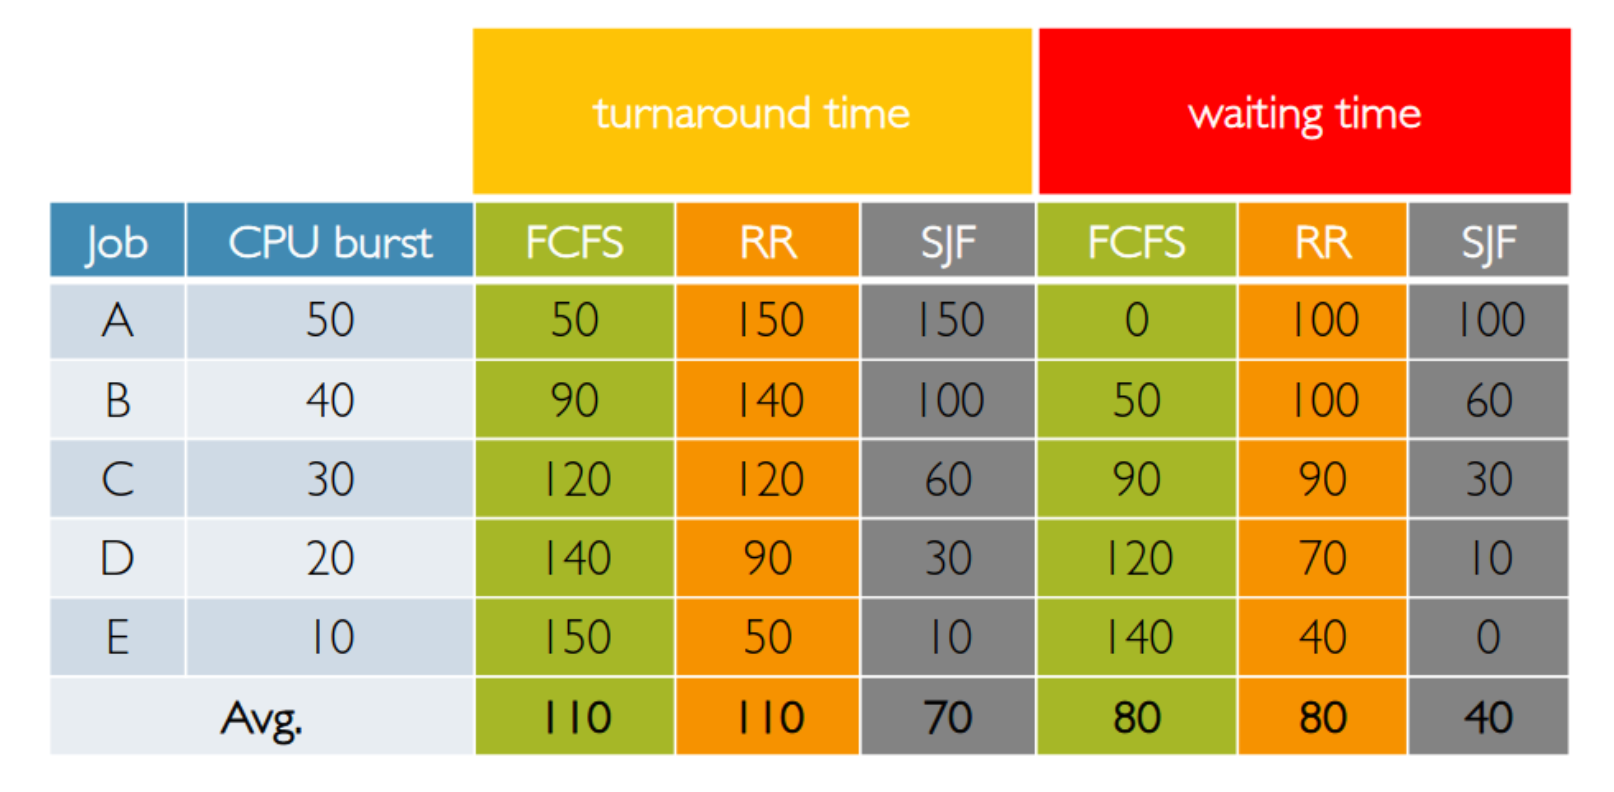
\includegraphics[width=0.5\textwidth,keepaspectratio]{{im/confronto3}}
        \caption{}    
    \end{center}
\end{figure}


\subsubsection{Priority Scheduling}
Nel \textbf{Priority Scheduling} a ciascun processo è assegnata una priorità e il processo eseguibile con la priorità più alta è quello cui è consentita l'esecuzione. Per impedire che i processi ad alta priorità siano eseguiti \textbf{indefinitamente}, lo scheduler può abbassare la priorità del processo attualmente in esecuzione a ogni scatto del clock (cioè a ogni interrupt). Se questa azione fa sì che la sua \textbf{priorità} vada al di sotto di quella del proceso successivo, avviene uno scambio di processo. In alternativa a ciascun processo può essere assegnato uno slice massimo in cui può essere eseguito.\par 
Le priorità possono essere assegnate in due modi:
\begin{itemize}
    \item Internamente, ossia assegnate dall'OS in base a determinati criteri (ad esempio il CPU burst medio, il rateo di attività tra CPU e I/O, risorse utilizzate, \dots)
    \item Esternamente, ossia assegnate dall'utente in base all'importanza del job o di altri criteri.
\end{itemize}\par

Un semplice algoritmo che offre un buon servizio ai processi I/O bound è quello di impostare la priorità a 1/$f$, dove $f$ è la frazione dell'ultimo quanto usao dal processo. Un processo che ha usato uno solo dei suoi 50 ms di slice avrà una prioria 50, mentre un processo che sia stato eseguito per 25 ms prima di bloccarsi avrà priorità 2; un processo che abbia usato tutto lo slice avrà priorità 1.

Il priority scheduling può essere sia \textbf{non-preemptive} sia \textbf{preemptive}.

\subsubsection*{Problemi}
Il Priority Scheduling può soffrire di starvation, dove un job di bassa priorità rimane in attesa perenne poiché altri job hanno sempre una priorità maggiore. Tali job potrebbero essere eseguiti eventualmente quando il carico del sistema è minore o dopo che il sistema stesso vada in crash, venga spento o venga riavviato. 
Come contromisura alla starvation viene utilizzato l'\textit{aging}, ossia l'incremento della priorità di un job in base al suo tempo in attesa, finché essi non verranno eventualmente schedulati.

\subsubsection{Multilevel Queue (MLQ)}








\pagebreak

\section{Sincronizzazione tra Processi/Thread}
%-------------------------------------------------------%
\pagebreak

\section{Gestione della Memoria}
%-------------------------------------------------------%
\pagebreak

\section{Gestione dei Sistemi di I/O}
%-------------------------------------------------------%
\pagebreak

\section{File System}
%-------------------------------------------------------%
\pagebreak

\section{Advanced Topics}


\end{document}

